%% The openany option is here just to remove the blank pages before a new chapter
\documentclass[11pt,openany]{book}
\usepackage[utf8]{inputenc}
\usepackage[utf8]{vietnam}
\usepackage{subcaption}
\usepackage{graphicx}
\usepackage{kantlipsum}
\usepackage{amsfonts}
\usepackage{amsmath}
\usepackage{float}
\usepackage{algorithm}
\usepackage{algorithmic}
\usepackage{hyperref}
\usepackage{tabularx}
\usepackage{diagbox}
\usepackage{slashbox}
\usepackage{lscape}
\usepackage{multirow}
\usepackage{longtable}
\usepackage{biblatex}
\addbibresource{mybib.bib}
\title{Communicating Multi-UAV System for cooperative SLAM-based Exploration}

\usepackage{pagenote}
\setcounter{chapter}{0}

%% End notes to be printed as sections at the
%% end of each chapter.
\renewcommand*{\notedivision}{\section*{\notesname}}
\renewcommand*{\pagenotesubhead}[1]{}


%%%%%%%%%%%%% For customising the endnote markers. Comment these out if you don't want them.
% To prefix each note number with the chapter number
\renewcommand{\thepagenote}{\thechapter-\arabic{pagenote}}

% To have a slightly different formatting for the endnote numbers in the text -- smaller text, sans-serif, square brackets
\renewcommand\notenumintext[1]{\space{\footnotesize\sffamily[FN-#1]}}

% To have a slightly different formatting for the endnote numbers in the notes section. Just the square brackets and sans-serif; normal size.
\renewcommand\notenuminnotes[1]{{\sffamily[FN-#1] }}

% If you want a different name/heading for the end notes
\renewcommand{\notesname}{End Notes}
%%%%%%%%%%%%% End customisation

%% THIS LINE IS MANDATORY
\makepagenote

\begin{document}
\begin{titlepage}
    \begin{center}
        \small
        TRƯỜNG ĐẠI HỌC BÁCH KHOA HÀ NỘI\\
        \vspace{0.2cm}
        \LARGE
        \textbf{VIỆN ĐIỆN TỬ - VIỄN THÔNG}\\
        \vspace{1.5cm}
        
\includegraphics[scale=0.3]{assets/logo.png}\\
        \vspace{1.5cm}
        \LARGE
        BÁO CÁO GIỮA KỲ\\
        \vspace{0.5cm}
        \Huge
        \textbf{ĐIỆN TỬ TƯƠNG TỰ II \\ DỊCH TÀI LIỆU}
        \vspace{1cm}
        \Large
        \begin{center}
            \begin{tabular}{ l l }
                \textbf{Nhóm}        & 49            \\
                \textbf{Sinh viên 1} & Tạ Hoàng Việt \\
                                     & 20172916      \\
                \textbf{Sinh viên 2} & Hồ Huy Hoàng  \\
                                     & 20172581
            \end{tabular}
        \end{center}
        \vspace{1cm}
        \normalsize
        Hà Nội, 06/2021
    \end{center}
\end{titlepage}
\tableofcontents
\listoffigures
\listoftables
\newpage
\thispagestyle{plain}
\addcontentsline{toc}{chapter}{Mở đầu}
\begin{center}
    \Huge
    \textbf{Mở đầu}
    \vspace{1cm}
\end{center}
% TODO: add introduction here
Tài liệu này được dịch lại từ bài báo "\textbf{Communicating Multi-UAV System for cooperative SLAM-based Exploration}", chương \textbf{3} và \textbf{4}.\\\\
Trong báo cáo này, chúng tôi sẽ đề xuất một chiến lược phối hợp khám phá nhiều robot để thăm dò và lập bản đồ các khu vực rộng lớn, từ đó xây dựng mô hình 3D cho không gian. Chiến lược được sử dụng để chỉ định robot đến mục tiêu và một hàm tiện ích được áp dụng để ước tính mức độ quan tâm của việc tiếp cận mục tiêu đó. Sau đó, một chiến lược dựa trên vai trò \textit{leader} sẽ phân công robot thực hiện mục tiêu.\\\\
Ngoài ra, chúng tôi cũng giải quyết vấn đề con của mạng MRS. Đầu tiên liên quan đến cấu trúc mạng là các đặc điểm cần được đảm bảo, trong khi đó, vấn đề thứ hai là chỉ ra sự phân phối địa lý của các nút mạng hay còn gọi là cấu trúc liên kết. Cấu trúc mạng đề xuất dựa trên việc áp dụng mạng lưới cùng với giao thức BATMAN. Kết quả đạt được rất khả quan, cải thiện hơn so với mạng Ad Hoc cơ bản.
\chapter{Khám phá phối hợp}
\section{Giới thiệu}
Việc thăm dò và lập bản đồ các khu vực rộng lớn là một lĩnh vực nghiên cứu tích cực trong lĩnh vực robot trên không. Nó bao gồm việc xây dựng mô hình 3D đại diện cho không gian làm việc khi rô bốt tiến triển bên trong nó. Gần đây, chủ đề quan trọng trong vấn đề thăm dò là việc triển khai hợp tác nhiều robot hứa hẹn nâng cao hiệu suất so với thăm dò bằng robot đơn lẻ.\\\\
Trong chương này, chúng tôi giải quyết vấn đề của các chiến lược thăm dò hợp tác mà không có kiến thức ưu tiên về môi trường. Chúng tôi sẽ cố gắng trả lời câu hỏi: Tiếp theo mỗi robot nên di chuyển đến đâu?
\section{Công việc có liên quan}
Gần đây, một số công trình đã đề xuất các giải pháp thăm dò bằng cách sử dụng các đội nhiều robot để giảm thời gian nhiệm vụ và tăng khả năng mở rộng \cite{bautin2012strategie}, \cite{jensen2013rolling}, \cite{yan2014team}. Do đó, thách thức là phải có sự hợp tác chặt chẽ giữa các đại lý trong hệ thống trong khi duy trì liên lạc \cite{rooker2007multi}. Vì vậy, các phương pháp tiếp cận hiện có có thể được tập trung hóa, nghĩa là, một robot trong thiết bị chịu trách nhiệm giao các mục tiêu \cite{burgard2000collaborative}. Trong \cite{schmuck2017multi}, một máy chủ trung tâm với nhiều tài nguyên tính toán được sử dụng để nhận, xử lý, tối ưu hóa và gửi lại thông tin cho các rô bốt khác. Các tác phẩm khác, chẳng hạn như \cite{yuan2010cooperative},\cite{sheng2006distributed}, sử dụng các phương pháp tiếp cận phân tán trong đó mỗi robot chọn mục tiêu của riêng mình. Một xu hướng khác là chuyển từ hành vi khám phá cá nhân sang hành vi hợp tác khi rô bốt không thể hội tụ đến mức tối thiểu cục bộ với tỷ lệ đáp ứng \cite{wu2012robust}. Trong \cite{konolige2003map}, các tác giả đề xuất xem xét bốn khả năng có tính đến tương tác của rô bốt để xây dựng bản đồ phân tán. Các tình huống liên quan là: không tương tác (các robot không nằm trong phạm vi giao tiếp của nhau), tạo giả thuyết (có sự tương tác giữa các robot nhưng chúng không biết vị trí tương ứng của mình), giả thuyết xác minh (có sự tương tác giữa các robot và họ đề xuất giả thuyết về vị trí của mình) và khám phá phối hợp (có sự tương tác giữa các robot và chúng chia sẻ bản đồ của mình).
\subsection{Phân công robot đến mục tiêu}
Thuật toán ánh xạ được thực hiện trong khi rô bốt cố gắng tiếp cận mục tiêu. Vì vậy, để lập bản đồ môi trường điện tử, mục tiêu cần được lựa chọn cẩn thận. Có rất nhiều chiến lược gán mục tiêu cho một robot tới một mục tiêu. Phần lớn chúng tập trung và sử dụng hàm chi phí để tính toán tiện ích của việc đạt được mục tiêu.\\\\
Trong nhiệm vụ Greedy \cite{yamauchi1998frontier}, mỗi robot chọn một mục tiêu tùy thuộc vào chức năng chi phí của nó mà không cần phối hợp với các robot khác. Do đó, một mục tiêu có thể được truy cập bởi các robot khác nhau. Để giải quyết vấn đề này, có thể loại bỏ các mục tiêu đã chọn trước khi được người khác xem xét chuyển nhượng bằng cách sử dụng tính năng Phát sóng về tính đủ điều kiện tại địa phương (BLE) \cite{werger2000broadcast} còn được gọi là Phép gán lặp lại. Tuy nhiên, phương pháp này không nhất thiết tạo ra giải pháp tối ưu vì nó phụ thuộc vào thứ tự của robot.\\\\
Phương pháp K-means \cite{solanas2004coordinated} bao gồm việc phân chia môi trường để khám phá thành các khu vực có cùng số lượng rô bốt, sau đó, chỉ định một rô bốt đến khu vực gần nhất nơi nó sẽ chọn mục tiêu từ các biên giới tùy thuộc vào hàm chi phí.\\\\
Phương pháp Hungarian \cite{deb1999multi} đề nghị bởi \cite{kuhn2005hungarian}, giải quyết công việc giao nhiệm vụ được viết dưới dạng $n \times n$ ma trận $C$ ở $c_{i,j}$ là chi phí của nhiệm vụ $j$ giao cho công nhân $i$. Bài tập tối ưu được tìm thấy với độ phức tạp về thời gian $O(n^3)$. Thuật toán này yêu cầu số lượng công nhân bằng số lượng nhiệm vụ không thể được đảm bảo. Ngoài ra, các rô bốt hoặc mục tiêu tưởng tượng có thể được thêm vào để đáp ứng giả định và được bỏ qua sau đó trong lựa chọn.\\\\
Các tác giả trong \cite{nanjanath2006dynamic} trình bày một phương pháp dựa trên đấu giá để giao nhiệm vụ cho một nhóm robot. Việc phân phối các nhiệm vụ được thực hiện bằng hình thức đấu giá ngược giá lần đầu có nghĩa là người bán đấu giá là người mua. Mỗi nhiệm vụ được bán đấu giá theo mức độ ưu tiên. Sau đó, đấu giá viên lựa chọn người trả giá tốt nhất và giao nhiệm vụ cho người trả giá tương ứng. Thuật toán này thích nghi tốt với các môi trường động, nơi các chướng ngại vật bất ngờ có thể ngăn cản rô-bốt tiếp cận mục tiêu.\\\\
Trong \cite{zhao1996genetic}, \cite{leigh2007using}, một thuật toán di truyền được sử dụng để giao nhiệm vụ cho robot một cách tối ưu. Đây là một bài toán khó NP vì nó được coi là một bài toán đóng gói thùng đa loại hai chiều tổng quát.\\\\
Các tác giả trong \cite{faigl2012goal} phản đối một cách tiếp cận mới được gọi là Bài toán nhân viên bán hàng đi du lịch nhiều nơi (MTSP) để phân công robot với mục tiêu trong bài toán khám phá nhiều robot. Nó bao gồm việc phân cụm một môi trường, xác định chi phí khoảng cách TSP cho mỗi cặp cụm robot, chỉ định mục tiêu từ cụm không trống và xác định mục tiêu cuối cùng cho các cụm trống. Cách tiếp cận này được so sánh với phương pháp tham lam, lặp đi lặp lại và phương pháp Hungarian. MTSP đưa ra các kết quả cạnh tranh về tổng số yêu cầu tính toán và số lượng robot ngày càng tăng.\\\\
Trong \cite{kulich2015comparison}, việc so sánh một số chiến lược phân công được sử dụng cho hệ thống nhiều robot được thực hiện. Các chiến lược được so sánh bao gồm phương pháp Hungarian, Greedy, phương pháp BLE và phân cụm K-means. Kết quả cho thấy rằng phương pháp Hungarian tốt hơn các phương pháp khác trong phần lớn các trường hợp. Không giống như phương pháp Hungarian, phép gán lặp đi lặp lại có thể được thực hiện trong một môi trường phân tán. Ngoài ra, các phương pháp Hungary nặng về mặt tính toán so với thuật toán Greedy đơn giản được ưu tiên trong kịch bản áp dụng.
\subsection{Hàm tiện ích}
Hầu hết việc robot đạt đến mục tiêu được dựa trên một hàm tiện ích được định nghĩa là các lợi ích mà robot phải đạt được, tính đến cả mục tiêu của nhiệm vụ đề ra\cite{burgard2000collaborative}. Công việc đề xuất trong \cite{benavides2016multi} trình bày một chức năng tiện ích mới có tính đến chi phí di chuyển đến mục tiêu và tiện ích kết nối. Điều này cho phép giao dịch giữa việc giảm thiểu số lượng thời gian thăm dò và kết nối. Để tăng tốc độ vận tốc, các tác giả trong \cite{cieslewski2017rapid} đề xuất một kỹ thuật lựa chọn biên giới nhanh chóng để chọn mục tiêu từ thực địa của robot. Cách tiếp cận này giảm thiểu thời gian nhiệm vụ tổng thể bằng cách giảm thiểu sự thay đổi vận tốc của robot. Tuy nhiên, cách tiếp cận này làm tăng tổng chiều dài đường dẫn đi. Trong \cite{heng2015efficient}, tối đa hóa mô hình tái tạo được ưa chuộng trong thời gian nhiệm vụ. Hơn nữa, cách tiếp cận được đề xuất giải quyết đồng thời các vấn đề thăm dò và bảo hiểm để tối đa hóa tính đầy đủ của mô hình tái tạo. Trong khi ở \cite{simmons2000coordination}, mục đích là tối đa hóa tiện ích của các mục tiêu giảm thiểu khả năng chồng chéo trong việc tăng thông tin giữa các thành viên của đội tàu. Tiện ích đạt được mục tiêu phụ thuộc về cơ bản về mục đích của nhiệm vụ trong khi tính đến một số ràng buộc bổ sung như thời gian, tính đầy đủ của bản đồ, cảm biến hạn chế và phạm vi giao tiếp, hoặc số lượng robot.
\section{Đề xuất chiến lược thăm dò}
\subsection{Tổng quát}
Trong một hệ thống nhiều UAV, chiến lược thăm dò cần phải hợp tác để tối đa hóa hiệu quả. Mục tiêu chính được đề xuất ở đây, là hợp tác lựa chọn các khu vực cụ thể để được khám phá đồng thời bằng cách tiếp cận dựa trên biên giới. Thông thường, điều này được thực hiện bằng cách chọn mục tiêu ứng viên và gán chúng cho mỗi robot một cách được tối ưu hóa. Hình \ref{fig:3.1} cho thấy quá trình thăm dò đường ống được đề xuất được thực hiện bởi mỗi UAV.
\begin{figure}[H]
    \centering
    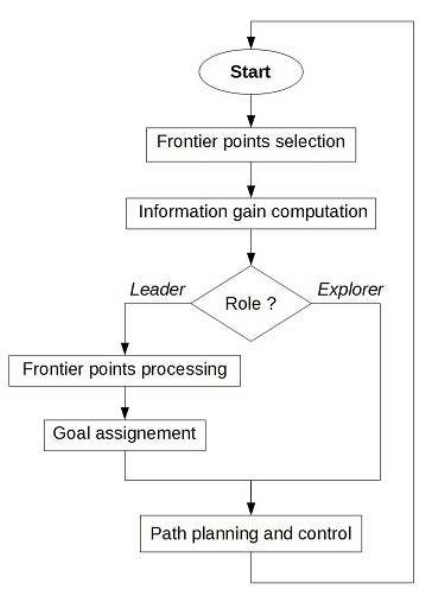
\includegraphics[scale=0.6]{assets/3_1.png}
    \caption{Đề xuất quá trình thăm dò đường ống.}
    \label{fig:3.1}
\end{figure}
Mỗi UAV chọn các điểm biên giới của bản đồ cục bộ được xây dựng trong bước SLAM.Sau đó, nó tính toán thông tin tương ứng của các điểm này.Nếu vai trò của UAV là một \textit{explorer}, nó sẽ thụ động chờ cho đến khi nhận được hướng dẫn; khác, nếu nó hoạt động như một \textit{leader}, nó sẽ xử lý các điểm biên giới được thu thập, và sẽ chỉ định một mục tiêu cho mỗi robot trong nhóm. Đưa ra một mục tiêu, UAV sẽ lên kế hoạch cho một đường dẫn cụ thể để đạt được nó.\\\\
Trong các bước này, cấu trúc bản đồ phát triển từ bản đồ lưới 2D dự kiến thu được từ mô-đun bản đồ và nội địa hóa, thông qua các điểm biên giới trong quá trình lựa chọn biên giới, sau đó các mục tiêu ứng cử viên trong bước xử lý biên giới, đến một tập các mục tiêu được chọn để đạt được. Sự phát triển của cấu trúc bản đồ được minh họa trong hình \ref{fig:3.2}. Thuật toán \ref{alg:3.1} mô tả các bước chính được thực hiện trong quá trình thăm dò.
\begin{algorithm}
    \caption{Chiến lược khám phá để phối hợp đa UAV}
    \label{alg:3.1}
    \begin{algorithmic}[1]
        \STATE From cell $\mathbf{l}_l \in \mathcal{L}$, select frontier points $\mathbf{f}_{i,j} \in \mathcal{F}$ and compute their respective information gain $\mathit{\mathbf{I}}(\mathbf{f}_{i,j})$.
        \STATE Process frontier points $\mathbf{f}_{i,j}$ to get candidate goals $\mathbf{t}_k \in \mathcal{G}$ (See Algorithm \ref{alg:3.2})
        \STATE Assign UAV$_i$ with target $k$ (See Algorithm \ref{alg:3.2}).
        \STATE Send targets to the corresponding robots.
    \end{algorithmic}
\end{algorithm}
\begin{figure}[H]
    \centering
    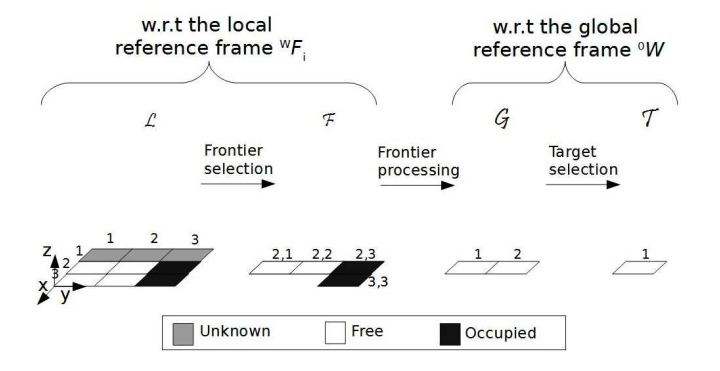
\includegraphics[scale=0.4]{assets/3_2.png}
    \caption{Tiến hóa cấu trúc bản đồ trong quá trình thăm dò: Từ các ô 2D $\mathcal{L}$ đến ô biên giới 2D. $\mathcal{F}$ để  cử  ứng viên biên giới / điểm $\mathcal{G}$ (mục tiêu ứng viên) đến 2D ô mục tiêu / điểm $\mathcal{T}$.}
    \label{fig:3.2}
\end{figure}
\subsection{Lựa chọn điểm biên giới}
Quá trình lựa chọn biên giới được sử dụng để định nghĩa biên giới của các vùng bị giới hạn bởi các chướng ngại vật hoặc không gian không xác định (Xem Hình \ref{fig:3.3}).
\begin{figure}[H]
    \centering
    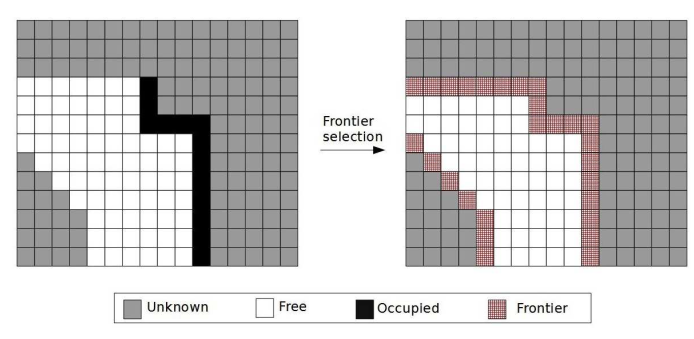
\includegraphics[scale=0.4]{assets/3_3.png}
    \caption{Các tế bào biên giới / điểm lựa chọn bản đồ lưới của phòng chiếm 2D.}
    \label{fig:3.3}
\end{figure}
Các tế bào biên giới $\mathbf{f}_{i,j} \in \mathcal{F}$ được chọn từ tập hợp các ô $\mathcal{L}(\mathcal{F}\subset \mathcal{L})$ sao cho chúng là:
\begin{itemize}
    \item Tự do $\mathbf{l}_f$ và liền kề với một unknown.
    \item Được dán nhãn là đã bị chiếm $\mathbf{l}_o$. Các ô bị chiếm $\mathbf{l}_o$ được coi là các tế bào biên giới để có thể thực hiện xử lý biên giới trong bước tiếp theo. Chúng không thể được chọn làm mục tiêu và sẽ bị loại bỏ sau.
\end{itemize}
Tại hình \ref{fig:3.2}, Các ô biên giới là: $\mathbf{l}_f(2,1)$,$\mathbf{l}_f(2,2)$ , $\mathbf{l}_f(2,3)$, và $\mathbf{l}_f(3,3)$. Vì vậy, đối với một cụm $\mathcal{C}$ chứa UAV$_i$, các biên giới là:
\begin{equation} \label{eq:3.1}
    \mathcal{F}=\{\mathbf{f}_{i,1}(2,1),\mathbf{f}_{i,2}(2,2),\mathbf{f}_{i,3}(2,3),\mathbf{f}_{i,4}(3,3)\}
\end{equation}
\subsection{Tính toán Infomation gain}
Trong các phương pháp khám phá dựa trên biên giới, chỉ các tế bào liền kề với những tế bào không xác định có thể được định nghĩa là các điểm biên giới ứng cử viên và có khả năng được chọn làm mục tiêu. Qua đó, mức tăng thông tin được liên kết với từng người trong số chúng để ước tính tiện ích tiếp cận từng biên giới. Việc tăng thông tin tương ứng này có thể được định nghĩa trong các cách cư xử khác nhau tùy thuộc vào mục đích nhiệm vụ. Tác giả trong \cite{burgard2005coordinated} đề xuất sử dụng chức năng xác suất để giảm giá trị không đổi được chỉ định có tính đến khoảng cách tương đối với tư thế của UAV. Chiến lược này là chung và không tính đến các ô được cập nhật được cập nhật. Hướng tiếp cận được đề xuất trong \cite{heng2015efficient} ảnh hưởng đến information gain về số lượng các ô không xác định và không bị chặn trong chế độ xem FrusM của mục tiêu. Phương pháp này phụ thuộc vào ước tính thực tế của thông tin đạt được khi đến thăm tư thế được coi là. Tuy nhiên, nó đòi hỏi nhiều tính toán hơn.\\\\
Trong chiến lược đề xuất, information gain được phân bổ để nó xác định lượng các ô không xác định xung quanh mục tiêu (Xem Hình \ref{fig:3.4}). Nó là một giá trị đếm số lượng các ô được dán nhãn là không xác định $\mathbf{l}_u$ từ 48 ô xung quanh điểm biên giới.
\begin{figure}[H]
    \centering
    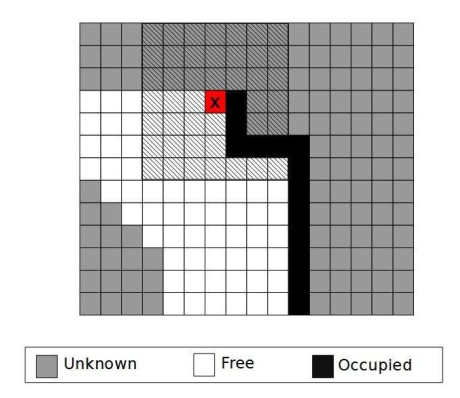
\includegraphics[scale=0.4]{assets/3_4.png}
    \caption{Tính toán information gain của một điểm biên x (ô đỏ). Các tế bào nở đại diện cho 48 tế bào xung quanh của điểm biên \textbf{x}. Information gain của \textbf{x} là: $\mathbf{I}(x)=25$.}
    \label{fig:3.4}
\end{figure}
\subsection{Xử lý điểm biên giới}
Tất cả các điểm biên giới $\mathbf{f}_{i,j} \in \mathcal{F}$ của UAV$_i$ Trong cụm $\mathcal{C}$ với $i \in [1..n_c]$, được thu thập. Điểm trong $\mathcal{F}$ sau đó được xử lý bằng thuật toán \ref{alg:3.2} để có được các điểm biên giới ứng cử viên được coi là mục tiêu ứng cử viên $\mathbf{t}_k \in \mathcal{G}$ với $k \in [1..n_g]$ (Xem Hình \ref{fig:3.2})
\begin{algorithm}[H]
    \caption{Thuật toán xử lý biên giới.}
    \label{alg:3.2}
    \hspace*{\algorithmicindent} \textbf{Input:} Frontier points $\mathbf{f}_{i,j} \in \mathcal{F}$ of UAV$_i$ with $i \in [1..n_c]$. \\
    \hspace*{\algorithmicindent} \textbf{Output:} Candidate targets $\mathcal{G}$
    \begin{algorithmic}[1]
        \STATE $p_u=\cup_{i=1}^{n_c}\mathbf{f}_{i,j}$.
        \STATE $p_i=\cap_{i=1}^{n_c}\mathbf{f}_{i,j}$.
        \STATE $\mathcal{G}=p_u\setminus p_i$.
        \STATE Delete the obstacle frontier points $\mathbf{f}_{i,j}(x,y)=\mathbf{l}_o(x,y)$ from $\mathcal{G}$.
        \RETURN $\mathcal{G}$.
    \end{algorithmic}
\end{algorithm}
Hình \ref{fig:3.5} hiển thị một ví dụ về xử lý biên giới với hai bản đồ của UAV để có được các mục tiêu ứng cử viên. Các điểm biên giới của chướng ngại vật $\mathbf{f}_{i,j}(x,y)=\mathbf{l}_o(x,y)$ – được dán nhãn là chiếm đóng (Occupied) - chỉ được giữ để tính toán giao điểm của các điểm biên. Chỉ các ô biên trống $\mathbf{l}_f$ có thể được coi là mục tiêu cho ứng cử viên.\\\\
Khi sử dụng điểm biên giới cục bộ thay vì bản đồ cục bộ, quy trình biên giới thay thế quy trình khớp bản đồ trong đó mục tiêu là để xóa các khu vực chồng chéo. Do đó, trong bước xử lý biên giới, các điểm biên giới thuộc các khu vực chồng chéo bị xóa.Do đó, sử dụng điểm biên giới cho phép tiết kiệm bộ nhớ quan trọng. Để tính các điểm biên giới thuộc về các khu vực chồng chéo (các bước 1, 2 và 3 trong thuật toán \ref{alg:3.2}), chúng tôi đề xuất hai cách tiếp cận với các hình dạng lồi và các giả định hình dạng lõm.
\subsubsection{Cách tiếp cận đầu tiên: Bản đồ dạng lồi}
Trong cách tiếp cận này, các hình dạng bản đồ được coi là convex, đơn giản hóa tính toán giao nhau trong thuật toán \ref{alg:3.3}. Hình \ref{fig:3.6} Hiển thị hai ví dụ về việc áp dụng thuật toán xử lý biên giới trong khi giả sử các hình lồi với hai và ba bản đồ của UAV.\\\\
Thuật toán này tương đối dễ dàng để áp dụng, nhưng kết quả cho thấy rằng nó không hoạt động tốt.Giả định lồi dẫn đến một số điểm biên giới chồng chéo sai.Do đó, một số khu vực chưa biết sẽ không được truy cập vì các điểm tương ứng của chúng được gỡ bỏ và do đó, sẽ không được chỉ định là mục tiêu.
\subsubsection{Cách tiếp cận thứ hai: Bản đồ hình dạng lõm}
Trong cách tiếp cận thứ hai, chúng tôi đưa ra giả định về các hình dạng lõm cho bản đồ của UAV để tính toán giao điểm của chúng trong thuật toán \ref{alg:3.4}. Hình \ref{fig:3.7} Hiển thị hai ví dụ về việc áp dụng thuật toán xử lý biên giới trong khi giả sử các hình lồi với hai và ba bản đồ của UAV.
\begin{figure}[H]
    \centering
    \begin{subfigure}[H]{0.6\linewidth}
        \centering
        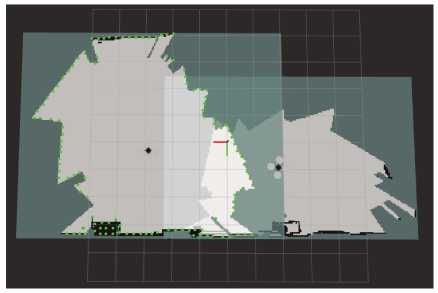
\includegraphics[width=\linewidth]{assets/3_5_a.png}
        \caption{{Các biên $\mathbf{f}_{1,j}$ của UAV$_1$}}
        \label{fig:3.5a}
    \end{subfigure}
    \begin{subfigure}[H]{0.6\linewidth}
        \centering
        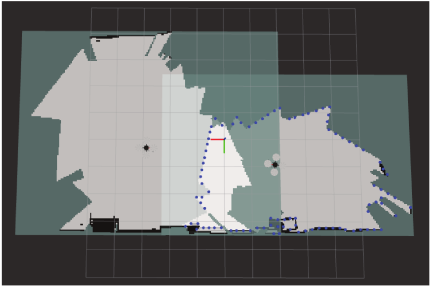
\includegraphics[width=\linewidth]{assets/3_5_b.png}
        \caption{{Các biên $\mathbf{f}_{2,j}$ của UAV$_2$}}
        \label{fig:3.5b}
    \end{subfigure}
    \begin{subfigure}[H]{0.6\linewidth}
        \centering
        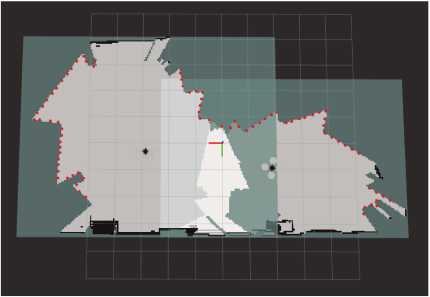
\includegraphics[width=\linewidth]{assets/3_5_c.png}
        \caption{{Mục tiêu đề cử $\mathcal{G}$}}
        \label{fig:3.5c}
    \end{subfigure}
    \caption{Ví dụ xử lý điểm biên giới: (a) và (b) đại diện cho các điểm biên giới của UAV$_1$ và UAV$_2$, tương ứng. (c) đại diện cho các mục tiêu ứng cử viên. Quá trình này bao gồm loại bỏ các điểm biên giới thuộc về các khu vực chồng chéo, và những điểm nằm liền kề với các chướng ngại vật.}
    \label{fig:3.5}
\end{figure}
\begin{algorithm}[H]
    \caption{Thuật toán tính toán giao nhau với giả định hình dạng lồi.}
    \label{alg:3.3}
    \hspace*{\algorithmicindent} \textbf{Input:} $Vect1, Vect2$ \\
    \hspace*{\algorithmicindent} \textbf{Output:} $Vect\_Final$
    \begin{algorithmic}[1]
        \FOR {$i \in Vect1$}
        \STATE $inf = 0, sup = 0$
        \FOR{ $j \in Vect2$}
        \IF {$Vect1(i).x < Vect2(i).x$}
        \STATE $inf++$;
        \ELSE
        \STATE $sup++$;
        \ENDIF
        \ENDFOR
        \IF {$inf>0$ and $sup>0$}
        \STATE $Vect\_inter.push\_back(Vect1(i))$
        \ENDIF
        \ENDFOR
        \FOR{$i \in Vect\_inter$}
        \STATE $inf=0,sup=0$;
        \FOR{$j \in Vect2$}
        \IF {$|Vect\_inter(i).x-Vect2(i).x| <0.5$}
        \STATE $inf++$;
        \ELSE
        \STATE $sup++$;
        \ENDIF
        \ENDFOR
        \IF {$inf>0$ and $sup>0$}
        \STATE $Vect\_Final.push\_back(Vect\_inter(i))$
        \ENDIF
        \ENDFOR
    \end{algorithmic}
\end{algorithm}
\begin{figure}[H]
    \centering
    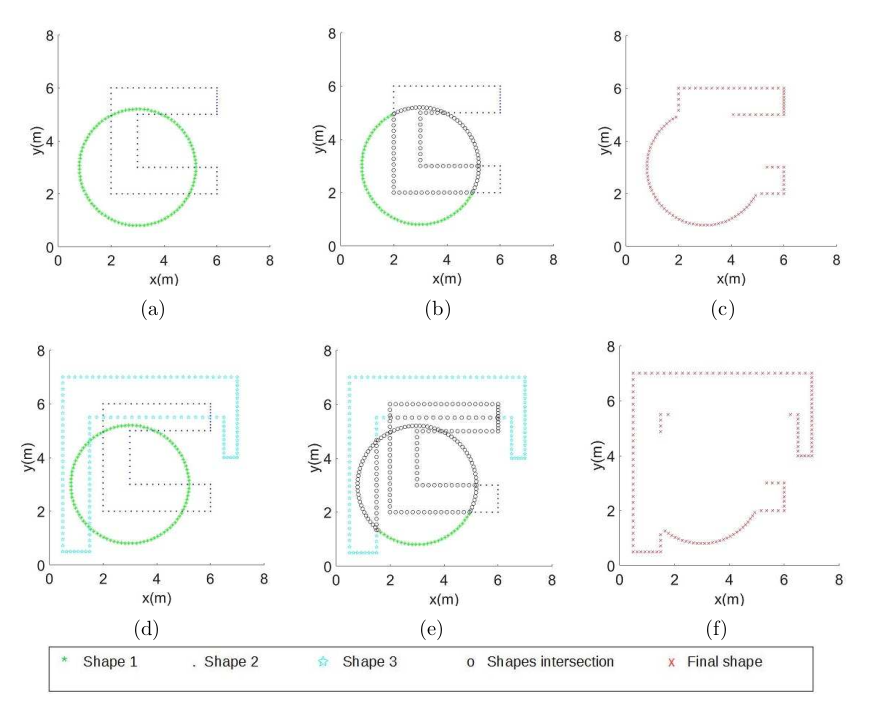
\includegraphics[scale=0.4]{assets/3_6.png}
    \caption{Xử lý điểm biên giới trong khi giả định hai hình dạng bản đồ lồi ở dòng đầu tiên và hình thứ ba trong dòng thứ hai. (a) và (d) đại diện cho hai và ba hình dạng bản đồ lồi, tương ứng, tương ứng; (b) và (e) đại diện cho các điểm biên giới chồng chéo (giao lộ); và (c) và (f) đại diện cho các điểm biên giới thu được sau khi xử lý (hình cuối cùng).}
    \label{fig:3.6}
\end{figure}
\begin{algorithm}[H]
    \caption{Thuật toán tính toán giao nhau với giả định hình dạng lồi.}
    \label{alg:3.4}
    \hspace*{\algorithmicindent} \textbf{Input:} $Vect1, Vect2$ \\
    \hspace*{\algorithmicindent} \textbf{Output:} $Vect\_Final$
    \begin{algorithmic}[1]
        \FOR {$i \in Vect1$}
        \STATE $inf = 0, sup = 0$
        \FOR{ $j \in Vect2$}
        \IF {$Vect1(i).x < Vect2(i).x -0.5$}
        \STATE $inf++$;
        \ELSIF {$Vect1(i).x>Vect2(i).x+0.5$}
        \STATE $sup++$;
        \ELSE
        \STATE $eq++$;
        \ENDIF
        \ENDFOR
        \IF {$inf>0$ and $sup>0$ or $eq>0$}
        \STATE $Vect\_inter.push\_back(Vect1(i))$
        \ENDIF
        \ENDFOR
        \FOR{$i \in Vect\_inter$}
        \STATE $inf=0,sup=0, eq=0$;
        \FOR{$j \in Vect2$}
        \IF {$|Vect\_inter(i).y-Vect2(i).y| <0.5$}
        \IF {$Vect\_inter(i).x<Vect2(i).x-0.5$}
        \STATE $inf++$;
        \ELSIF {$Vect1(i).x>Vect2(i).x+0.5$}
        \STATE $sup++$;
        \ELSE
        \STATE $eq++$;
        \ENDIF
        \ENDIF
        \ENDFOR
        \IF {($inf>0$ and $sup>0$) or $eq>0$}
        \STATE $Vect\_Final.push\_back(Vect\_inter(i))$
        \ENDIF
        \ENDFOR
    \end{algorithmic}
\end{algorithm}
\begin{figure}[H]
    \centering
    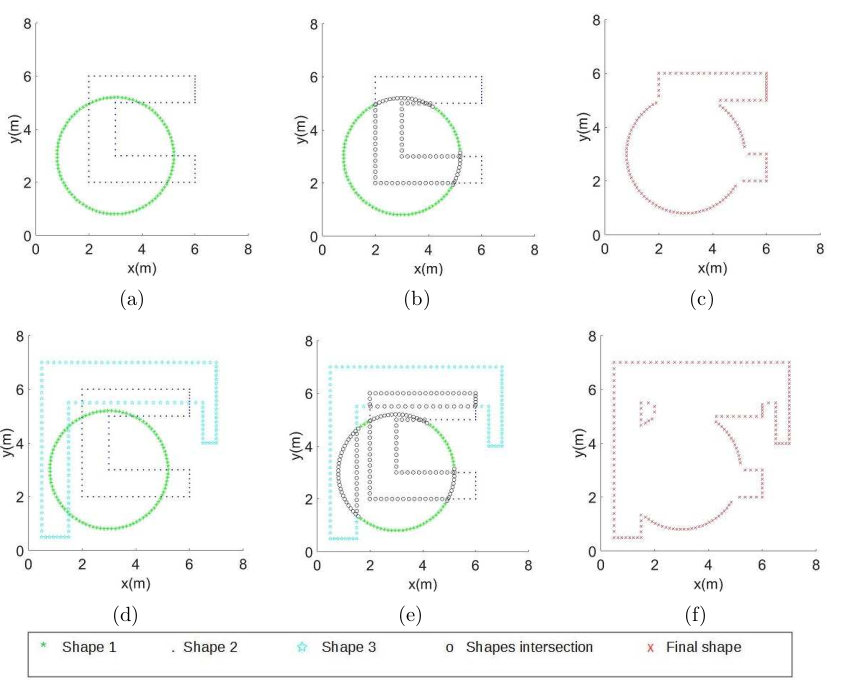
\includegraphics[scale=0.4]{assets/3_7.png}
    \caption{Xử lý điểm biên giới trong khi giả định hai hình dạng bản đồ lồi ở dòng đầu tiên và hình thứ ba trong dòng thứ hai. (a) và (d) đại diện cho hai và ba hình dạng bản đồ lồi, tương ứng, tương ứng; (b) và (e) đại diện cho các điểm biên giới chồng chéo (giao lộ); và (c) và (f) đại diện cho các điểm biên giới thu được sau khi xử lý (hình cuối cùng).}
    \label{fig:3.7}
\end{figure}
Kết quả cho thấy chỉ các điểm biên giới trong các khu vực chồng chéo được loại bỏ.Ngay cả khi một số điểm biên giới mơ hồ được đặt trong / bên trong hình dạng toàn cầu - có thể gây nhầm lẫn -, chúng không bị xóa.Thuật toán này, giả sử các hình dạng lõm, thực hiện tốt hơn so với trước đó giả định hình dạng lồi.Do đó, đối với chế biến biên giới, hình dạng của bản đồ địa phương được giả định lõm.
\subsubsection{Hàm tiện ích}
Hàm tiện ích được đề xuất trong công thức \ref{eq:3.2} nhằm mục đích tăng đồng thời tỷ lệ khu vực được khám phá và để giảm khoảng cách của từng UAV đến mục tiêu tương ứng. Hàm này cũng xem xét trung bình khoảng cách giữa mỗi robot trong nhóm và mục tiêu này để tối đa hóa khoảng cách giữa các robot.
\begin{equation}
    \mathbf{U}(UAV_i,t_j)=\mathbf{I}(t_j)exp(-\lambda.(dmin(\mathbf{P}_i,\mathbf{t}_j)+\frac{n_c-1}{d_{tot}})),
\end{equation}
trong đó UAV$_i$ được coi là robot, $\mathbf{t}_j \in \mathcal{G}$ và $\mathbf{I}(\mathbf{t}_j)$ tương ứng là mục tiêu ứng viên và mức tăng thông tin tương ứng của nó, $\lambda \in [0,1]$ là một tham số giao dịch, $n_c$ là số lượng UAV trong cụm $\mathcal{C}$, và $d_{tot} = \sum_{k=1, k\neq i}^{n_c}(dmin(\mathbf{P}_k),\mathbf{t}_j) $ là tổng của khoảng cách tối thiểu từ pose của UAV$_k$ $\mathbf{P}_k$ đến mục tiêu ứng viên $j$. Hàm tiện ích đề xuất được truyền cảm hứng từ \cite{heng2015efficient} và nó đã được trình bày trong các công việc của chúng tôi \cite{mahdoui2017cooperative},\cite{mahdoui2018cooperative}. Hàm này thực hiện sự đánh đổi giữa khám phá nhanh chóng với một bản đồ chính xác bằng cách sử dụng tham số điều chỉnh $\lambda$. Từ hình \ref{fig:3.8}, chúng ta có thể nhận thấy rằng với $\lambda$ lớn hơn, khoảng cách $d_{tot}$ ít quan trọng hơn. Do đó, việc thăm dò nhanh chóng một cách chính xác sẽ được ưu tiên hơn và ngược lại.\\\\
Về trường hợp đa UAV, hàm tiện ích dựa trên trung bình khoảng cách hàng xóm. Như thể hiện trong hình \ref{fig:3.8}, với information gain $\mathbf{I}(\mathbf{t}_j)=25$ và ba UAV trong cụm $(n_c=3)$; Một khoảng cách ngày càng tăng của UAV đến mục tiêu sẽ làm giảm hàm tiện ích. Trong khi đó, khoảng cách trung bình lớn hơn so với các UAV khác w.r.t. đến mục tiêu, tiện ích càng nhiều. Vì vậy, hàm có xu hướng chọn mục tiêu được coi là gần nhất với UAV ; Nhưng đồng thời, xa nhất từ những người khác.\\\\
Trong trường hợp một UAV duy nhất, chức năng tiện ích (xem công thức \ref{fig:3.3}) Có xu hướng chọn mục tiêu gần nhất với mức tăng tối đa thông tin:
\begin{equation}
    \mathbf{U}(UAV_i,\mathbf{t}_j)=\mathbf{I}(\mathbf{t}_j)exp(-\lambda.(dmin(\mathbf{P}_j,\mathbf{t}_j))),
\end{equation}
Tham số $d_{tot} = \sum_{k=1, k\neq i}^{n_c}(dmin(\mathbf{P}_k,\mathbf{t}_j)) $ đại diện cho tổng khoảng cách tối thiểu giữa mục tiêu $\mathbf{t}_j$ và các pose của hangf xóm $\mathbf{P}_k$ với $k \in [1..n_c]\setminus i$. Vì thế, nếu $\mathbf{t}_j$ có UAV lân cận quá xa, hàm tiện ích sẽ tăng lên, vì vậy $\mathcal{T}_j$ có nhiều khả năng được chọn.\\\\
Mục tiêu của hàm tiện ích là tìm max của $d_{tot}$. Chúng tôi phân biệt hai trường hợp là $d_{tot}$ có thể quá gần bằng 0 hoặc bằng nó:
\begin{figure}[H]
    \centering
    \begin{subfigure}[H]{0.4\linewidth}
        \centering
        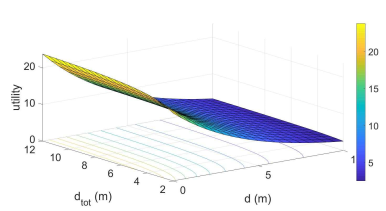
\includegraphics[width=\linewidth]{assets/3_8_a.png}
        \caption{{$\lambda=0.2$}}
        \label{fig:3.8a}
    \end{subfigure}
    \begin{subfigure}[H]{0.4\linewidth}
        \centering
        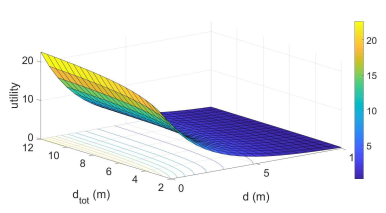
\includegraphics[width=\linewidth]{assets/3_8_b.png}
        \caption{{$\lambda=0.4$}}
        \label{fig:3.8b}
    \end{subfigure}
    \begin{subfigure}[H]{0.4\linewidth}
        \centering
        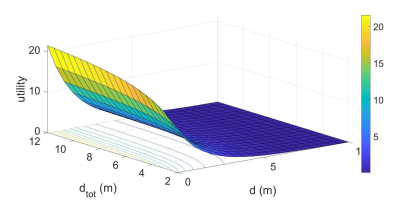
\includegraphics[width=\linewidth]{assets/3_8_c.png}
        \caption{{$\lambda=0.6$}}
        \label{fig:3.8c}
    \end{subfigure}
    \begin{subfigure}[H]{0.4\linewidth}
        \centering
        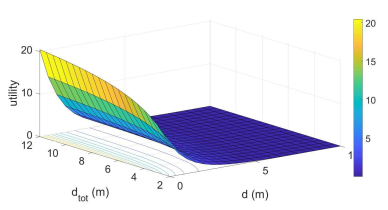
\includegraphics[width=\linewidth]{assets/3_8_d.png}
        \caption{{$\lambda=0.8$}}
        \label{fig:3.8d}
    \end{subfigure}
    \caption{{Hàm tiện ích thực hiện: $\mathbf{I}(t_j)=25, n_c=3, d_{tot} = \sum_{k=1, k\neq i}^{n_c}(dmin(\mathbf{P}_k,\mathbf{t}_j))$. Khoảng cách trung bình $d_{tot}$ giữa các UAV có giá trị tối thiểu khác 0 khi $n_c$ cũng khác 0.}}
    \label{fig:3.8}
\end{figure}
\begin{itemize}
    \item Không có hàng xóm. Trong trường hợp này, có một UAV trong hạm đội: $n_c=1$. Hàm tiện ích trong công thức \ref{eq:3.3} được sử dụng.
    \item Mục tiêu đề ra $\mathbf{t}_j$ và các pose của lân cận $\mathbf{P}_k$ với $k \in [1..n_c]\setminus i$ quá gần nhau. Trong trường hợp này $\mathbf{t}_j$ ít có khả năng được chọn.
\end{itemize}
Tuy nhiên, tham số $d_{tot}$ có thể có giá trị cao khi:
\begin{itemize}
    \item Có một UAV quá xa $\mathbf{t}_j$.
    \item Có một số UAV với khoảng cách tương đối ngắn từ $\mathbf{t}_j$.
\end{itemize}
Vì vậy, để tránh những tình huống mơ hồ này, giá trị trung bình của $d_{tot}$ được tính toán bằng $\frac{n_c}{d_{tot}}$.
\subsection{Quy trình phân công mục tiêu}
Để thực hiện phân công UAV đến mục tiêu thích hợp, tiện ích tiếp cận từng biên giới tiềm năng được xem xét. Quá trình phân công mục tiêu được mô tả trong thuật toán \ref{alg:3.5}.\\\\
Với mỗi UAV$_i$ , các tiện ích để đạt được tất cả các mục tiêu tiềm năng được tính toán. Mục tiêu $\mathbf{t}_g$ được tính từ hàm tối đa hóa tiện ích và phân công $\theta(UAV_i,\mathbf{t}_g)$ được đưa ra. Sau đó, các mục tiêu ứng cử viên còn lại $\mathcal{G}\setminus \mathcal{T}$ được lên kế hoạch để tránh chọn một mục tiêu quá gần $\mathbf{t}_g$ , ở vòng lặp tiếp theo. Cũng thế, $\mathbf{t}_g$ bị xóa bỏ từ $\mathcal{G}$ để tránh việc gán cùng một mục tiêu cho các robot khác nhau. Quá trình chuyển nhượng này được thực hiện cho các UAV có sẵn trong $\mathcal{C}$ theo cách tuần tự cho đến khi nhận được tất cả các mục tiêu được chỉ định $\mathbf{t}_g \in \mathcal{T}$ với $g \in [1..n_t]$ (Xem Hình \ref{fig:3.2})
\begin{algorithm}[H]
    \caption{Thuật toán gán mục tiêu.}
    \label{alg:3.5}
    \hspace*{\algorithmicindent} \textbf{Input:} {Candidate targets $\mathbf{t}_k \in \mathcal{G}, k \in [1..n_g]$ and their respective information gain $\mathbf{U}(\mathbf{t}_k)$, poses $\mathbf{P}_i$ of all robots in the considered cluster $\mathcal{C}$.}\\
    \hspace*{\algorithmicindent} \textbf{Output:} {$\theta(UAV_i,\mathbf{t}_g)$ assignment of UAV$_i$ with target $g$.}
    \begin{algorithmic}[1]
        \STATE $\mathcal{T}=\theta$
        \WHILE{no goal for UAV$_i$}
        \STATE Compute its corresponding utility of reaching each remaining candidate goal $\mathbf{U}(UAV_i,\mathbf{t}_k)$ with $\mathbf{t}_k \in \mathcal{G}\setminus \mathcal{T}$.
        \STATE $t_g=argmax_{t_k \in \mathcal{G}\setminus \mathcal{T}}(\mathbf{U}(UAV_i,\mathbf{t}_k))$.
        \STATE Schedule the information gain of the remaining candidates $\mathbf{t}_k \in \mathcal{G} \setminus \mathcal{T}$.
        \STATE $\mathcal{T}=\mathcal{T}\cup t_g$.
        \ENDWHILE
        \RETURN $\theta(UAV_i, \mathbf{t}_g)$ assignment.
    \end{algorithmic}
\end{algorithm}
\subsubsection{Điều kiện dừng}
Quá trình lựa chọn mục tiêu được thực hiện bởi mỗi cluster/group-\textit{leader} (nếu $n>n_c$ ) hoặc là fleet-\textit{leader} (nếu $n=n_c$). Nhiệm vụ này nhằm mục đích, hợp tác, phân phối robot trong môi trường để khám phá đồng thời các khu vực không xác định khác nhau. Miễn là các điểm biên giới tiềm năng vẫn có sẵn, \textit{leader} tiếp tục gán mục tiêu cho \textit{explorers} và họ cố gắng đạt được mục tiêu được giao. Khi \textit{leader} thông báo rằng không có mục tiêu ứng cử viên nào còn lại, điều đó có nghĩa là tất cả các môi trường đã được khám phá thành công và nhiệm vụ được thực hiện. Vì vậy, nó phải gửi lại cho \textit{explorers} một sự thừa nhận để ngăn chặn giả định tắc nghẽn.
\subsubsection{Tỉ lệ lặp}
Quá trình phân công mục tiêu được thực hiện tại mỗi vòng lặp. Tần suất gán các mục tiêu ảnh hưởng đến thời gian và hiệu quả của nhiệm vụ. Trong một cách tiếp cận phân tán, ngay khi UAV đạt được mục tiêu hiện tại, nó sẽ chọn một mục tiêu mới mà không cần tham khảo ý kiến người khác. Trong một cách tiếp cận tập trung, UAV đầu tiên đạt được mục tiêu hiện tại phải đợi cho đến khi những người khác đạt được mục tiêu tương ứng của họ. Đây có thể là một vấn đề ngay khi một trong số họ thất bại hoặc rời khỏi nhiệm vụ. Một khả năng khác là bắt đầu gán các mục tiêu sau khi UAV đạt được mục tiêu. Nhưng điều này có thể tạo ra các nhiệm vụ không đầy đủ. Trong chiến lược đề xuất, tần suất phân công hoặc tỷ lệ vòng lặp $r$ được xác định trước tùy thuộc vào trung bình thời gian để đạt được mục tiêu (Xem công thức \ref{eq:3.4}).
\begin{equation} \label{eq:3.4}
    r \in [\frac{s}{v_{i,max}},\frac{s}{v_{i,min}}]
\end{equation}
trong đó $s$ là phạm vi cảm biến tối đa vaf $v_i$ là vận tốc của UAV.
\subsubsection{Lên lịch với information gain}
Tăng thông tin của từng mục tiêu ứng cử viên còn lại $\mathbf{I}(\mathbf{t}_k)_{t-1}$ tại thời điểm $t-1$ với $\mathbf{t}_k \in \mathcal{G} \setminus \{t_g\}$, thuộc về phạm vi ngưỡng $[r_{min} , r_{max} ]$, được lên kế hoạch tại thời điểm $ t $ tùy theo khoảng cách của nó w.r.t. mục tiêu $t_g$ , sử dụng công thức \ref{eq:3.5}. Hình \ref{fig:3.9} đại diện cho một ví dụ về hình dạng chức năng được sử dụng để lên lịch để đạt được thông tin.Ví dụ cho thấy một hàm Gaussian với biên độ tương ứng với giá trị tối đa thông tin; một trung tâm tương ứng với vị trí mục tiêu $(\mathbf{t}_g(x), \mathbf{t}_g(y))$; và $\sigma_x$ và $\sigma_y$ nó lan rộng blob trong trục $x$ và $y$, tương ứng.
\begin{figure}[H]
    \centering
    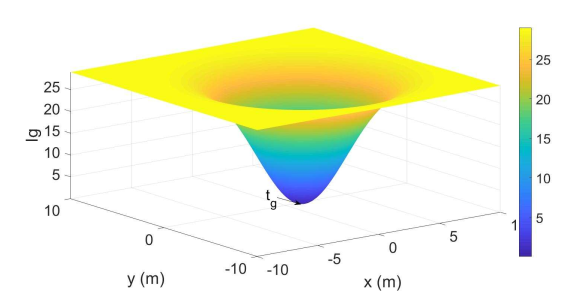
\includegraphics[scale=0.6]{assets/3_9.png}
    \caption{Ví dụ về hình dạng của hàm lên kế hoạch information gain($\mathbf{I}(\mathbf{t}_k)_{t-1}=29,(\mathbf{t}_g(x),\mathbf{t}_g(y))=(1.25,-0.275), \sigma_x=\sigma_y=3$).}
    \label{fig:3.9}
\end{figure}
\begin{equation}\label{eq:3.5}
    \mathbf{I}(\mathbf{t}_k)_t=\mathbf{I}(\mathbf{t}_k)_{t-1}(1-exp(-(\frac{(\mathbf{t}_k(x)-\mathbf{t}_g(x))^2}{2.\sigma_x^2}+\frac{(\mathbf{t}_k(y)-\mathbf{t}_g(y))^2}{2.\sigma_y^2}))),
\end{equation}
trong đó $\mathbf{t}_k(x)$ và $\mathbf{t}_k(y)$ là tọa độ mục tiêu ứng cử viên còn lại; $\mathbf{t}_g(x)$ và $\mathbf{t}_g(y)$ là tọa độ mục tiêu; và $\sigma_x$ và $\sigma_y$ là sự lây lan của blob. Khoảng cách của điểm biên giới nhỏ hơn $\mathbf{t}_k$ w.r.t. mục tiêu $\mathbf{t}_g$, information gain càng nhỏ. Khi giảm information gain, các mục tiêu ứng cử viên ít có khả năng được chọn và do đó, robot đảm bảo một khoảng cách nhất định trong số các mục tiêu trong tương lai của họ.
\subsection{Lên kế hoạch và kiểm soát đường dẫn}
Như được giải thích trong Phần 5.2 của Chương 1, UAV được giả định để điều hướng trong môi trường 2D đơn giản hóa với một giá trị $z$ cố định. Khối \textbf{6} trong Hình 1.6 chịu trách nhiệm lên kế hoạch cho một đường dẫn đến mục tiêu đã chọn và cố gắng tiếp cận nó. Những nhiệm vụ này được đảm bảo bởi gói \textit{move} cơ bản\footnote{Nguồn: \url{http://wiki.ros.org/move_base}}.\\\\
Đối với nhiệm vụ điều hướng, mỗi UAV duy trì một công cụ lập kế hoạch địa phương và toàn cầu cùng với một costmap địa phương và toàn cầu. Costmap là một lưới ô 2D $\mathcal{L}$ với bổ sung trong lạm phát bao gồm việc truyền các giá trị chi phí từ các tế bào bị chiếm đóng và giảm chúng bằng khoảng cách.CostMap toàn cầu có kích thước của bản đồ của UAV trong khi đó, costmap địa phương có một cửa sổ di chuyển kích thước cố định. Đưa ra một điểm khởi đầu - tư thế hiện tại - và điểm cuối - mục tiêu được chỉ định - trong costmap toàn cầu, công cụ lập kế hoạch toàn cầu tạo ra một kế hoạch sử dụng chức năng điều hướng được tính bằng thuật toán Dijkstra \cite{dijkstra1959note}. Nó bao gồm sau các tế bào tự do liền kề cho đến khi đạt được mục tiêu. Sau đó tính đến chi phí địa phương, công cụ lập kế hoạch cục bộ tạo ra các lệnh vận tốc cho căn cứ di động của UAV. Một hành vi quay trở lại cũng được thực hiện khi cần thiết để xóa chế độ xem của robot.\\\\
Mục tiêu được chỉ định bởi \textit{leader} được đảm bảo là thuộc về một khu vực không xác định bằng cách sử dụng chiến lược thăm dò. Quá trình lập kế hoạch quỹ đạo được thực hiện tại địa phương trên mỗi robot. Và vì UAV không trao đổi bản đồ địa phương của họ cũng như hợp nhất chúng, họ có khả năng xem lại các khu vực đã khám phá trong khi theo đường dẫn theo kế hoạch. Để giảm thiểu các vùng chồng chéo này trong quá trình điều hướng, ưu tiên được đưa ra cho các điểm biên giới $\mathbf{f}_{i,j}$ là một mục tiêu cho UAV$_i$ ngoài UAV$_k$ với $k \neq i$. Điều này giúp UAV duy trì cùng một hướng trong quá trình thăm dò. Các \textit{move} Gói cơ sở là một ngăn xếp điều hướng 2D. Tuy nhiên, để tránh trôi dạt trên trục $z$, một lệnh điều khiển được thêm vào để giữ cố định độ lớn $z$ (Xem hình \ref{fig:3.10}).
\begin{figure}[H]
    \centering
    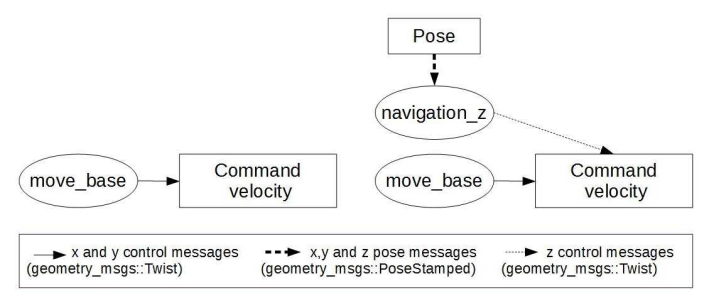
\includegraphics[scale=0.4]{assets/3_10.png}
    \caption{Từ ngăn xếp điều hướng 2D (trái) sang 3D (phải). \textit{Navigation} $z$ là một quá trình ROS được phát triển để cung cấp một lệnh điều khiển trên trục $z$.}
    \label{fig:3.10}
\end{figure}
\section{Kết quả và thảo luận}
Mô phỏng đã được thực hiện để đánh giá chiến lược thăm dò được đề xuất. Các thử nghiệm bổ sung trong khi sử dụng bản địa hóa tương đối đã được thực hiện để đo lường hiệu suất hệ thống. Các mô phỏng được thực hiện bởi Robot Operating System (ROS) chạy trên thiết bị 2.60GHz i7 Linux. Đối với mô phỏng bốn cánh quạt, mô hình AR-Drone\footnote{Source: \url{http://wiki.ros.org/ardrone_autonomy}} được trang bị máy ảnh RGB-D theo cấu hình tìm hướng chuyển tiếp, được sử dụng. Một môi trường không xác định được tạo ra bằng cách sử dụng mô phỏng \textit{Gazebo}. Số lượng robot được sử dụng để đánh giá được giới hạn ở ba, tuy nhiên, kiến trúc hệ thống được đề xuất không bị hạn chế với một số robot cố định.
\subsection{Điều chỉnh thông số}
Để đánh giá hiệu quả về chiến lược thăm dò, chúng tôi sẽ chạy một số thử nghiệm để đặt cấu hình tham số đầy đủ nhất.
\subsubsection{Tham số trade-off $\lambda$}
Hàm tiện ích (Xem công thức \ref{eq:3.2}) được sử dụng trong chiến lược thăm dò có thể được điều chỉnh, sử dụng tham số trade-off $\lambda$, giữa khám phá nhanh chóng và một bản đồ chi tiết.\\\\
Hình \ref{fig:3.11} hiển thị các kết quả khác nhau trong khi thay đổi tham số này. Bằng cách tăng $\lambda$, thông tin thu được khi đạt được mục tiêu ưu tiên về khoảng cách và do đó, chi phí cho nó tăng lên và ngược lại. Vì thế, khi $\lambda$ nhỏ, khoảng cách di chuyển là nhỏ và vì vậy thời gian thăm dò nhỏ. Mặc dù, một số lần trong nhiệm vụ, giá trị $\lambda$ cao cho thấy tỷ lệ thăm dò cao hơn so với những giá trị nhỏ hơn.
\begin{figure}[H]
    \centering
    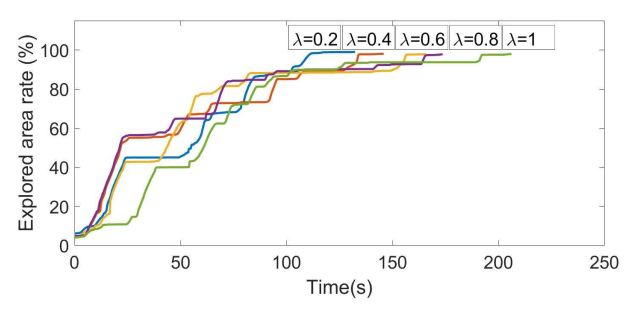
\includegraphics[scale=0.5]{assets/3_11.png}
    \caption{Ảnh hưởng của việc thay đổi tham số trade-off $\lambda$ qua thời gian thăm dò.}
    \label{fig:3.11}
\end{figure}
\subsubsection{Tỉ lệ vòng lặp $r$}
Tỷ lệ tần số hoặc vòng lặp $r$ của nhiệm vụ mục tiêu cũng có thể ảnh hưởng đến hiệu suất thời gian thăm dò. Giá trị $r$ thay đổi để tính đến vận tốc robot $\mathbf{v}_i$ và phạm vi tối đa của cảm biến $s$. Tác động của việc thay đổi tỷ lệ vòng lặp được đánh giá trong Hình \ref{fig:3.12}.
\begin{figure}[H]
    \centering
    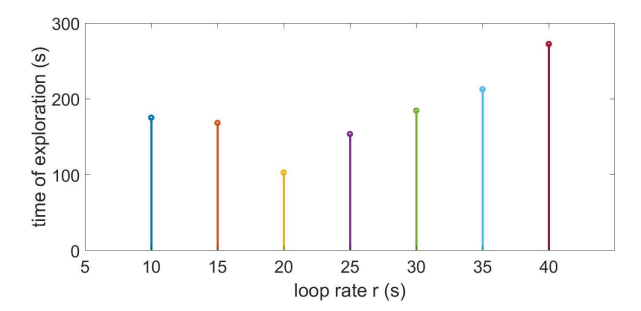
\includegraphics[scale=0.5]{assets/3_12.png}
    \caption{Thời gian khám phá trong khi thay đổi tỷ lệ vòng lặp $r$.}
    \label{fig:3.12}
\end{figure}
Cho vận tốc robot $\mathbf{v}_i=\{0.1,0.3\}m.s^{-1}$ và phạm vi cảm biến tối đa $s=4m$, tỉ lệ vòng lặp thay đổi trong $r \in [10,40]$. Tham số này không nên quá nhỏ để cho phép robot đạt được mục tiêu; cũng không quá lớn để ngăn chặn thời gian chờ đợi dài cho nhiệm vụ cần đạt tiếp theo.
\subsubsection{Thông số chung}
Dựa vào kết quả ở Hình \ref{fig:3.11} và Hình \ref{fig:3.12}, tương ứng, $\lambda$ cho bằng $0.2$ vaf $r$ là $20s$ để tối đa hóa tỷ lệ khu vực được khám phá trong khi giảm thiểu thời gian nhiệm vụ. Các tham số mô phỏng được tóm tắt trong Bảng \ref{tab:3.1}.
\begin{table}[H]
    \centering
    \caption{Thông số chung.}
    \label{tab:3.1}
    \begin{tabular}{|l|l|}\hline
        \makebox[5em]{\textbf{Parameter}}                  & \makebox[5em]{\textbf{Value}}
        \\\hline
        RGB-D horizental FoV                               & $\pi/ 3$                      \\\hline
        Trade-off parameter $\lambda$                      & 0.2                           \\\hline
        RGB-D maximum range $s (m)$                        & 4                             \\\hline
        Min distance among frontiers $d (m)$               & 0.3                           \\\hline
        Occupancy grid resolution $(m)$                    & 0.05                          \\\hline
        Range to schedule the $\lg[\sigma_x,\sigma_y] (m)$ & $[3,3]$                       \\\hline
        Loop rate $l (s)$                                  & 20                            \\\hline
        Enviroment dimension $(m^2)$                       & $8 \times 8$                  \\\hline
        Linear velocity $v_i (m.s^{-1})$                   & $[0.1,0.3]$                   \\\hline
        Angular velocity $w_i (rad.s^{-1})$                & $[0.1,0.3]$                   \\\hline
    \end{tabular}
\end{table}
\subsection{Trình bày chiến lược khám phá}
Chiến lược thăm dò được đề xuất đã được đánh giá về mặt phân phối robot trong môi trường, tỷ lệ chồng chéo, thời gian thăm dò và toàn bộ khoảng cách di chuyển của mỗi robot.
\subsubsection{Bản đồ tiến hóa trong nhiệm vụ}
Trong khi đạt được mục tiêu được giao nhiệm vụ tương ứng, mỗi robot phụ trách việc tạo bản đồ lưới chi tiết của khu vực đã truy cập để có được bản đồ toàn cầu về môi trường. Hình \ref{fig:3.13} minh họa sự phát triển của bản đồ lưới chiếm dụng 3D được xây dựng lại vào các thời điểm khác nhau trong nhiệm vụ. Lưu ý rằng khi độ phủ sóng đạt $99\%$ sẽ tốn rất nhiều thời gian.\\\\
Hình \ref{fig:3.14} hiển thị sự phát triển của bản đồ lưới địa phương 2D dự kiến tương ứng của hai robot trong một nhiệm vụ thăm dò hợp tác xã. Bản đồ lưới 2D dự kiến toàn cầu cũng được tạo và đại diện để đánh giá (quy trình khớp lưới chiếm dụng được giới thiệu trong thuật toán 2.1 trong Chương 2 được sử dụng). Vị trí ban đầu của robot UAV$_1$ là $(1,0,0)$ và của UAV$_2$ là $(1,-3,0)$. Mặc dù có một vị trí ban đầu tương đối chặt chẽ, chiến lược đề xuất đã lan rộng hiệu quả robot để UAV$_1$ chịu trách nhiệm về phía bên trái của môi trường và UAV$_2$ bên phải.
\subsubsection{Sự tiến hóa điểm biên trong nhiệm vụ}
Mục tiêu được chọn từ các điểm biên giới ứng cử viên xác định các cạnh của môi trường không được khám phá trước đó. Những ứng cử viên này được chọn từ các điểm biên giới cuối cùng của mỗi UAV trong hạm đội (Xem Hình \ref{fig:3.15}). Trong nhiệm vụ thăm dò, kích thước bản đồ địa phương tăng lên, dẫn đến số lượng điểm biên giới cục bộ ngày càng tăng. Khi bắt đầu thăm dò, số lượng điểm biên giới tiềm năng tăng lên, nhưng ngay khi thăm dò tiến hóa kịp thời, số lượng của chúng giảm. Vào cuối nhiệm vụ, khi tất cả các môi trường được khám phá, không nên để lại điểm biên giới tiềm năng.
\subsubsection{Quỹ đạo của UAV trong nhiệm vụ}
Hình \ref{fig:3.16} hiển thị bản đồ được khám phá với các quỹ đạo bằng cách sử dụng một, hai và ba UAV. UAV cố gắng khám phá môi trường đầy đủ trong khi tránh các khu vực đã khám phá. Một cách hợp tác, mỗi UAV phụ trách truy cập một khu vực bằng cách đạt được mục tiêu thuộc về một môi trường không khám phá. Những mục tiêu này được chỉ định bởi \textit{Leader}, ngay cả khi các pose ban đầu của UAV tương đối gần, trải rộng hiệu quả của chúng vào các khu vực chưa biết. Bản đồ toàn cầu bao gồm sự chồng chất của tất cả các bản đồ địa phương của tất cả các UAV.
\begin{figure}[H]
    \centering
    \begin{subfigure}[H]{0.3\linewidth}
        \centering
        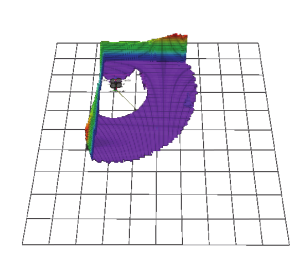
\includegraphics[width=\linewidth]{assets/3_13_a.png}
        \caption{{$3\%$ rate $(5s).$}}
        \label{fig:3.13a}
    \end{subfigure}
    \begin{subfigure}[H]{0.3\linewidth}
        \centering
        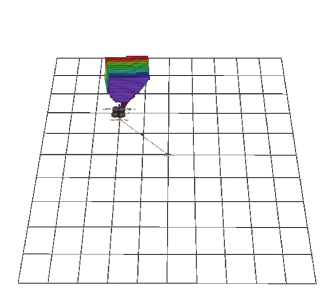
\includegraphics[width=\linewidth]{assets/3_13_b.png}
        \caption{{$20\%$ rate $(28s).$}}
        \label{fig:3.13b}
    \end{subfigure}
    \begin{subfigure}[H]{0.3\linewidth}
        \centering
        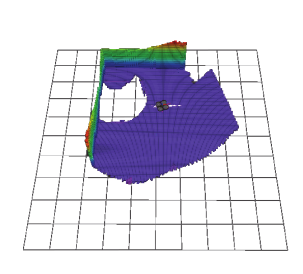
\includegraphics[width=\linewidth]{assets/3_13_c.png}
        \caption{{$31\%$ rate $(50s).$}}
        \label{fig:3.13c}
    \end{subfigure}
    \begin{subfigure}[H]{0.3\linewidth}
        \centering
        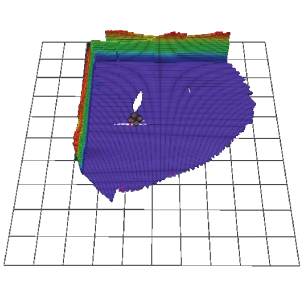
\includegraphics[width=\linewidth]{assets/3_13_d.png}
        \caption{{$40\%$ rate $(69s).$}}
        \label{fig:3.13d}
    \end{subfigure}
    \begin{subfigure}[H]{0.3\linewidth}
        \centering
        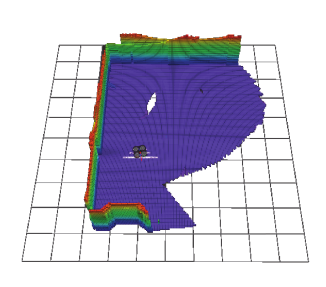
\includegraphics[width=\linewidth]{assets/3_13_e.png}
        \caption{{$50\%$ rate $(75s).$}}
        \label{fig:3.13e}
    \end{subfigure}
    \begin{subfigure}[H]{0.3\linewidth}
        \centering
        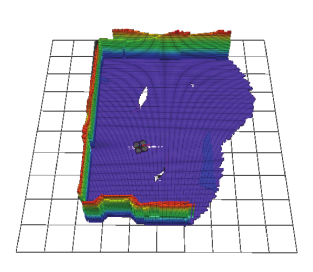
\includegraphics[width=\linewidth]{assets/3_13_f.png}
        \caption{{$60\%$ rate $(83s).$}}
        \label{fig:3.13f}
    \end{subfigure}
    \begin{subfigure}[H]{0.3\linewidth}
        \centering
        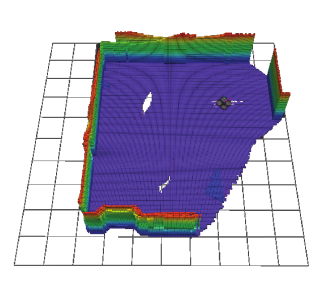
\includegraphics[width=\linewidth]{assets/3_13_g.png}
        \caption{{$70\%$ rate $(98s).$}}
        \label{fig:3.13g}
    \end{subfigure}
    \begin{subfigure}[H]{0.3\linewidth}
        \centering
        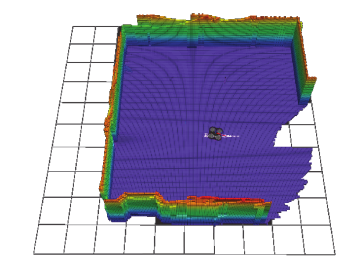
\includegraphics[width=\linewidth]{assets/3_13_h.png}
        \caption{{$81\%$ rate $(127s).$}}
        \label{fig:3.13h}
    \end{subfigure}
    \begin{subfigure}[H]{0.3\linewidth}
        \centering
        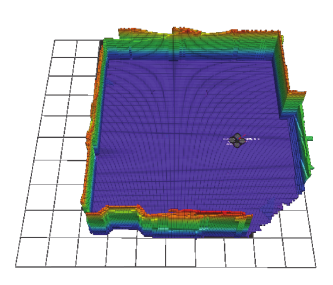
\includegraphics[width=\linewidth]{assets/3_13_i.png}
        \caption{{$90\%$ rate $(133s).$}}
        \label{fig:3.13i}
    \end{subfigure}
    \begin{subfigure}[H]{0.3\linewidth}
        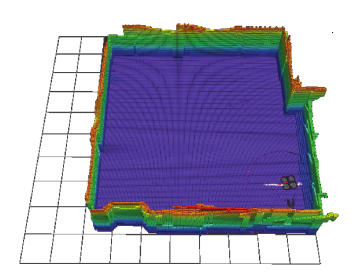
\includegraphics[width=\linewidth]{assets/3_13_j.png}
        \caption{{$99\%$ rate $(202s).$}}
        \label{fig:3.13j}
    \end{subfigure}
    \caption{Tỷ lệ không gian khám phá trong thời gian cho một UAV.}
    \label{fig:3.13}
\end{figure}
\begin{figure}[H]
    \centering
    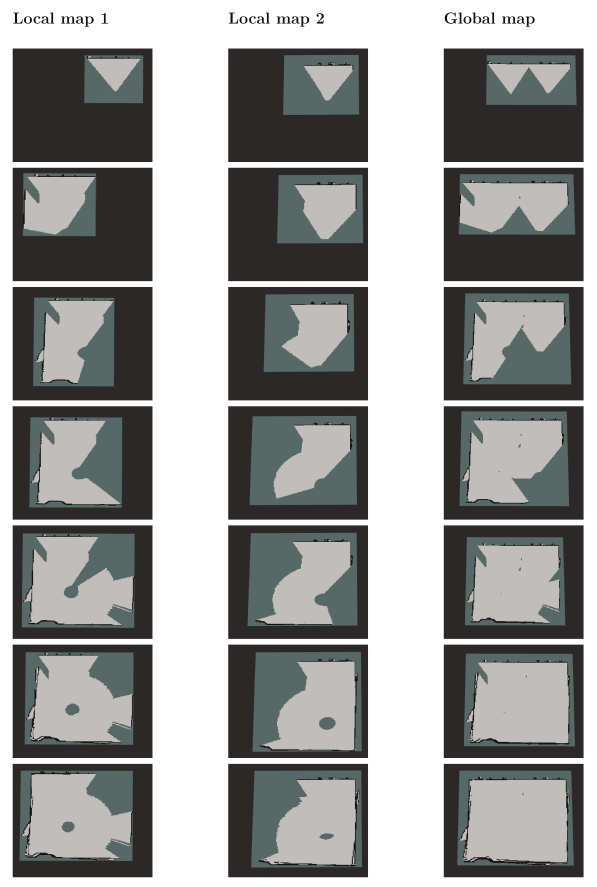
\includegraphics[scale=0.5]{assets/3_14.png}
    \caption{Phối hợp thăm dò bằng hai robot. Cột 1, 2 và 3 cho thấy sự phát triển của bản đồ địa phương của UAV$_1$, các UAV$_2$ và bản đồ toàn cầu theo thời gian, tương ứng.}
    \label{fig:3.14}
\end{figure}
\begin{figure}[H]
    \centering
    \begin{subfigure}[H]{0.7\linewidth}
        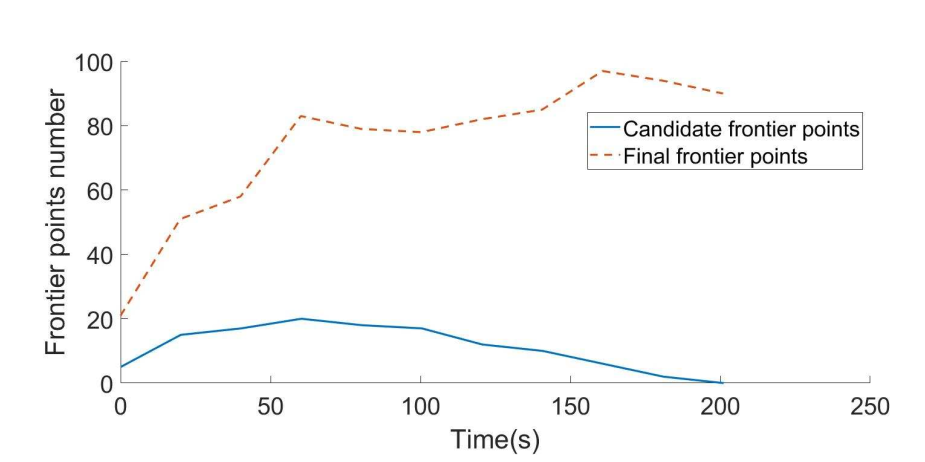
\includegraphics[width=\linewidth]{assets/3_15_a.png}
        \caption{{Một UAV.}}
        \label{fig:3.15a}
    \end{subfigure}
    \begin{subfigure}[H]{0.7\linewidth}
        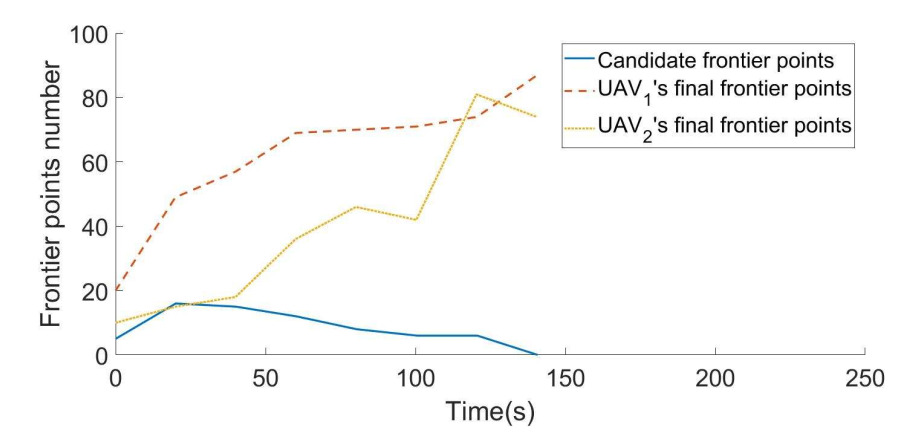
\includegraphics[width=\linewidth]{assets/3_15_b.png}
        \caption{{Hai UAV kết hợp.}}
        \label{fig:3.15b}
    \end{subfigure}
    \begin{subfigure}[H]{0.7\linewidth}
        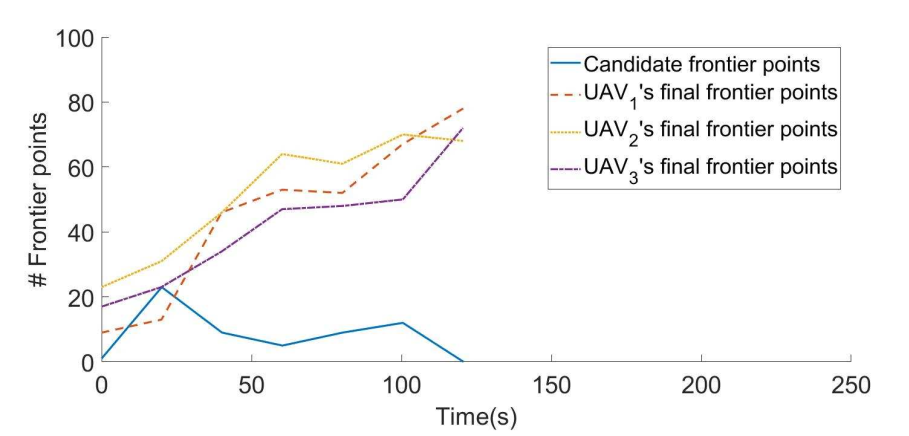
\includegraphics[width=\linewidth]{assets/3_15_c.png}
        \caption{{Ba UAV kết hợp.}}
        \label{fig:3.15c}
    \end{subfigure}
    \caption{Sự phát triển của ứng cử viên và số điểm biên giới cuối cùng trong quá trình thăm dò hợp tác.}
    \label{fig:3.15}
\end{figure}
\begin{figure}[H]
    \centering
    \begin{subfigure}[H]{0.5\linewidth}
        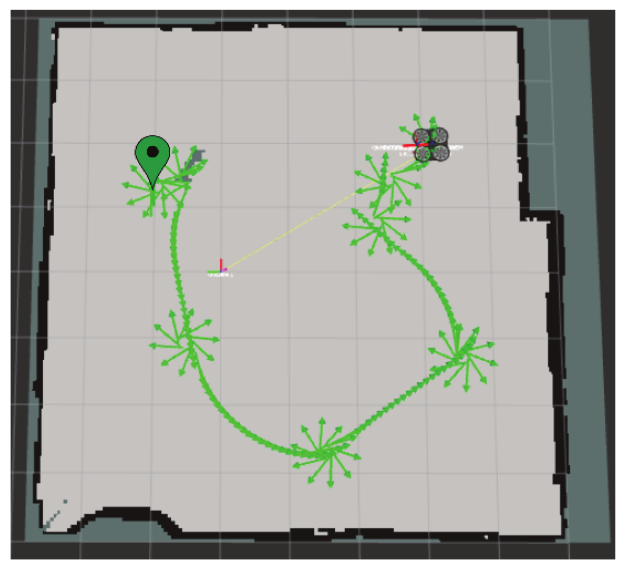
\includegraphics[width=\linewidth]{assets/3_16_a.png}
        \caption{{Một UAV.}}
        \label{fig:3.16a}
    \end{subfigure}
    \begin{subfigure}[H]{0.5\linewidth}
        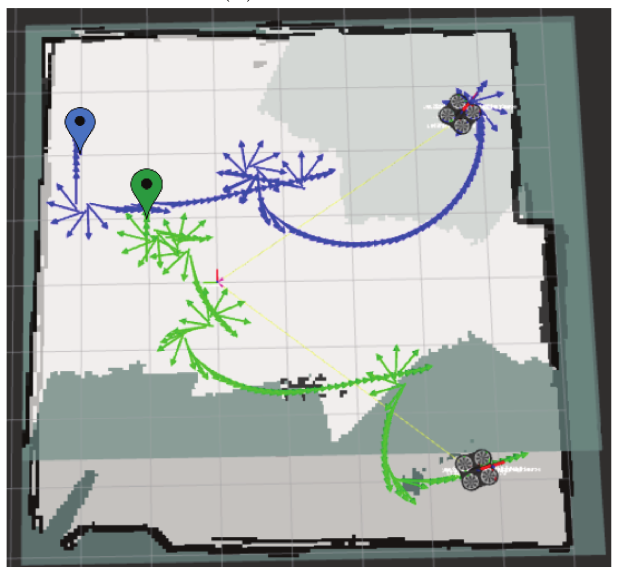
\includegraphics[width=\linewidth]{assets/3_16_b.png}
        \caption{{Hai UAV kết hợp.}}
        \label{fig:3.16b}
    \end{subfigure}
    \begin{subfigure}[H]{0.5\linewidth}
        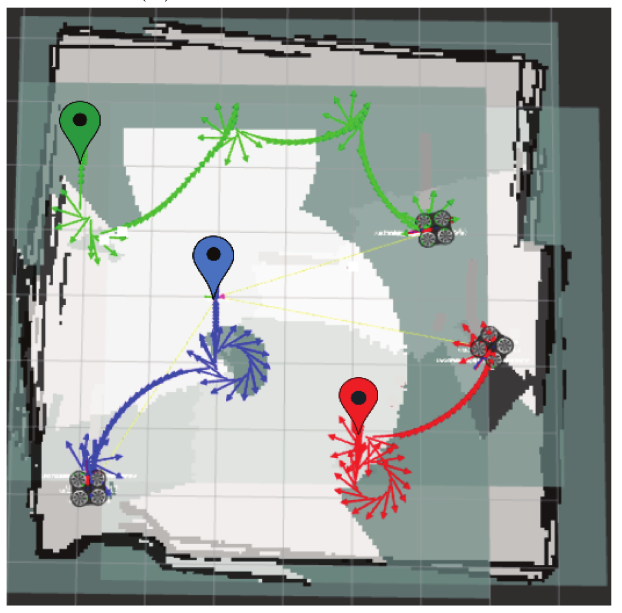
\includegraphics[width=\linewidth]{assets/3_16_c.png}
        \caption{{Ba UAV kết hợp.}}
        \label{fig:3.16c}
    \end{subfigure}
    \caption{Dự kiến bản đồ 2D trong một cuộc thám hiểm phối hợp với một nhóm một, hai và ba UAV. Các dấu hiệu và mũi tên màu xanh lá cây, xanh dương và đỏ xác định, tương ứng, vị trí ban đầu và quỹ đạo của UAV1, UAV2 và UAV3.}
    \label{fig:3.16}
\end{figure}
\subsubsection{Đánh giá nhiệm vụ mục tiêu: Phân phối robot trong môi trường}
Quá trình phân công mục tiêu được thực hiện theo thuật toán được mô tả trong Phần 3.6. Tuy nhiên, sau khi chỉ định mục tiêu cho robot đầu tiên trong danh sách, cùng một mục tiêu hoặc một mục tiêu khác gần với nó có thể được gán cho robot thứ hai trong danh sách. Để khắc phục những vấn đề này, mức tăng thông tin của các mục tiêu ứng cử viên còn lại được lên lịch. Điều này cho phép loại bỏ một mục tiêu đã được chỉ định và giữ một khoảng cách nhất định giữa mục tiêu mới và phần trước được chỉ định.\\\\
Giả sử rằng một mục tiêu được gán cho robot đầu tiên trong danh sách cụm. Hình \ref{fig:3.17} hiển thị mục tiêu được chọn cho robot thứ hai khi một bài tập tuần tự được thực hiện:
\begin{itemize}
    \item Không cần xử lý điểm biên giới nữa (Xem Hình \ref{fig:3.17b}). Do đó, mục tiêu tương tự được gán cho hai robot khác nhau.
    \item Trong khi loại bỏ mục tiêu được gán từ các điểm biên giới ứng cử viên còn lại (Xem Hình \ref{fig:3.17c}). Do đó, mục tiêu thứ hai tương đối gần với chỉ định đầu tiên.
    \item Trong khi lên lịch trình thông tin tăng sau mỗi lần gán mục tiêu (Xem Hình \ref{fig:3.17d}). Do đó, các mục tiêu được chỉ định được cách nhau vào môi trường.Lợi ích thông tin được lên lịch theo lịch trình Eq. \ref{eq:3.5}. Giá trị thông tin tăng lên với khoảng cách đến mục tiêu ứng viên $\mathbf{t}_g$.
\end{itemize}
Quá trình phân công mục tiêu đôi khi có thể không tối ưu vì nó phụ thuộc vào thứ tự của robot trong danh sách.Ví dụ, giả sử robot UAV$_i$ và UAV$_j$ có cùng một nhiệm vụ mục tiêu tốt nhất t k sao cho nó đạt được tiện ích tối đa so với các điểm biên giới ứng viên, nơi Eq.\ref{eq:3.6} và Eq. \ref{eq:3.7} được xác minh.
\begin{equation}\label{eq:3.6}
    \mathbf{t}_k=argmax_{t_m}\mathbf{U}(UAV_i,\mathbf{t}_m)
\end{equation}
with $\mathbf{t}_m \in \mathcal{G}$.
\begin{equation}\label{eq:3.7}
    \mathbf{t}_k=argmax_{t_n}\mathbf{U}(UAV_j, \mathbf{t}_n)
\end{equation}
with $\mathbf{t}_n \in \mathcal{G}$.\\
UAV$_i$ have another candidate frontier point $\mathbf{t}_l$ with:
\begin{equation}\label{eq:3.8}
    \mathbf{\mathit{U}}(UAV_i, \mathbf{t}_k) > \mathbf{\mathit{U}}(UAV_i,\mathbf{t}_l) > \mathbf{\mathit{U}}(UAV_j, \mathbf{t}_k)
\end{equation}

\begin{figure}[H]
    \centering
    \begin{subfigure}[H]{0.6\linewidth}
        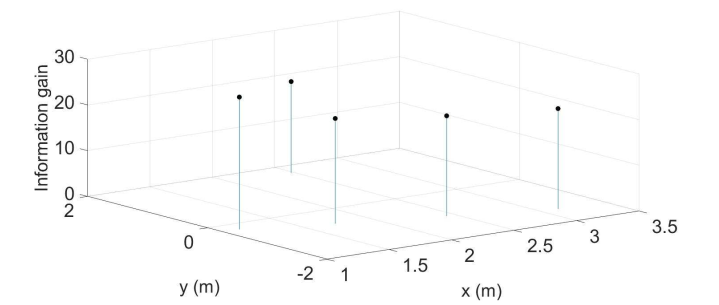
\includegraphics[width=\linewidth]{assets/3_17_a.png}
        \caption{{Mục tiêu ứng viên.}}
        \label{fig:3.17a}
    \end{subfigure}
    \begin{subfigure}[H]{0.6\linewidth}
        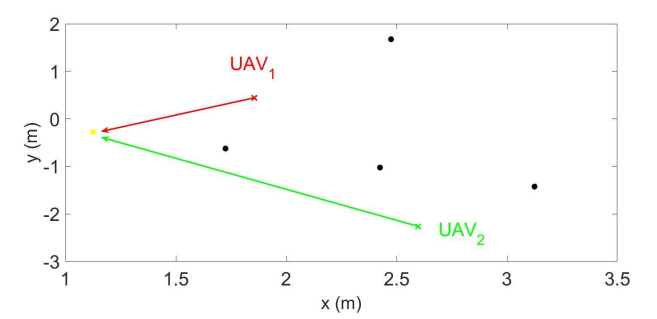
\includegraphics[width=\linewidth]{assets/3_17_b.png}
        \caption{{Trường hợp 1.}}
        \label{fig:3.17b}
    \end{subfigure}
    \begin{subfigure}[H]{0.6\linewidth}
        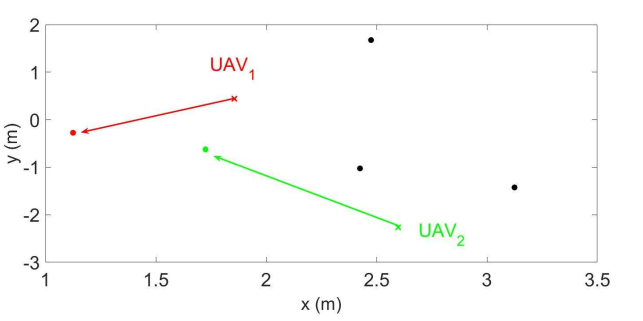
\includegraphics[width=\linewidth]{assets/3_17_c.png}
        \caption{{Trường hợp 2.}}
        \label{fig:3.17c}
    \end{subfigure}
    \begin{subfigure}[H]{0.6\linewidth}
        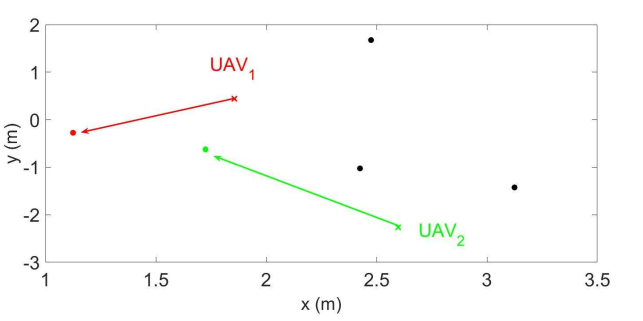
\includegraphics[width=\linewidth]{assets/3_17_c.png}
        \caption{{Trường hợp 3.}}
        \label{fig:3.17d}
    \end{subfigure}
    \caption{Nhiệm vụ mục tiêu: Sau khi chỉ định một mục tiêu để UAV$_1$ , một mục tiêu được chỉ định theo cách liên tiếp để UAV$_2$ . (a) đại diện cho các điểm biên giới ứng cử viên với mức tăng thông tin tương ứng của họ.(b), (c) và (d) đại diện, tương ứng, nhập mục tiêu khi: Không có quy trình nào khác được thực hiện cho các mục tiêu ứng cử viên còn lại; mục tiêu của UAV$_1$ được loại bỏ khỏi các mục tiêu ứng cử viên còn lại và; việc đạt được thông tin của các mục tiêu ứng cử viên còn lại được lên lịch.}
    \label{fig:3.17}
\end{figure}
Vì vậy, giải pháp tối ưu sẽ là gán $\mathbf{t}_l$ cho UAV$_i$ và $\mathbf{t}_k$ cho UAV$_j$ . Nhưng nếu UAV$_i$ là đầu tiên trong danh sách, $\mathbf{t}_k$ được gán cho nó và một điểm biên lai khác với ít tiện ích hơn $\mathbf{t}_k$, được chỉ định cho UAV$_j$. Do đó, giải pháp với việc phân công mục tiêu tuần tự không phải lúc nào cũng tối ưu.\\\\
Để khắc phục vấn đề này, tất cả các số kết hợp có thể xảy ra $\frac{n_g!}{n_g!(n_g-n_c)!}$ với $n_g$ số lượng mục tiêu ứng cử viên và $n_c$ số lượng robot, cần phải được xem xét. Điều này tăng đáng kể thời gian tính toán bằng cách tăng số lượng robot. Do đó, trong thuật toán được đề xuất, nhiệm vụ tuần tự được ưa chuộng về việc tính toán tất cả các hoán vị có thể.
\subsubsection{Khám phá đánh giá tỷ lệ không gian}
Đánh giá này nhằm định lượng lượng không gian khám phá trong nhiệm vụ. Hình \ref{fig:3.18} cho thấy tỷ lệ không gian được khám phá được thực hiện bởi mỗi UAV trong FL EET.Càng nhiều UAV trong môi trường, tỷ lệ thăm dò càng ít yêu cầu.Một robot không cần phải tiếp tục khám phá một khu vực nếu nó đã được khám phá bởi một khu vực khác.Do đó, thời gian nhiệm vụ giảm đáng kể.
\subsubsection{Đánh giá tỷ lệ chồng chéo}
Việc sử dụng một quy trình phân công mục tiêu hiệu quả sẽ giới hạn sự chồng chéo được tạo. Trong Hình \ref{fig:3.19}, thời gian phát triển của sự chồng chéo được đánh giá bằng hai robot hợp tác. Sự chồng chéo trải qua một sự gia tăng đáng kể vào cuối cuộc thăm dò để đạt được $33\%$. Điều này được giải thích bởi sự gần gũi của các bản đồ địa phương vào cuối nhiệm vụ để điền chính xác bản đồ lưới toàn cầu.
\begin{figure}[H]
    \centering
    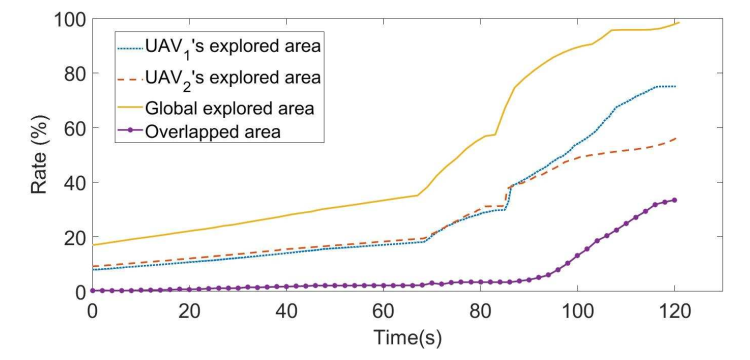
\includegraphics[scale=0.4]{assets/3_19.png}
    \caption{Tỷ lệ khu vực được khám phá và chồng chéo bằng cách sử dụng hai UAV hợp tác.}
    \label{fig:3.19}
\end{figure}
\subsubsection{Đánh giá khoảng cách di chuyển}
Để đánh giá hiệu quả hiệu suất chiến lược thăm dò về khoảng cách di chuyển của mỗi UAV, các lần chạy khác nhau với một, hai và ba UAV đã được thực hiện khi tỷ lệ khu vực được khám phá đạt gần như $99\%$. Hình \ref{fig:3.20} cho thấy khoảng cách di chuyển của mỗi UAV trong hạm đội trong nhiệm vụ.
\begin{figure}[H]
    \centering
    \begin{subfigure}[H]{0.7\linewidth}
        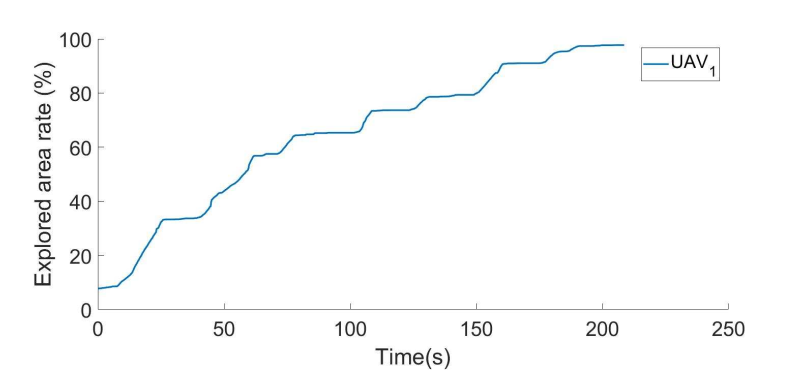
\includegraphics[width=\linewidth]{assets/3_18_a.png}
        \caption{{Một UAV.}}
        \label{fig:3.18a}
    \end{subfigure}
    \begin{subfigure}[H]{0.7\linewidth}
        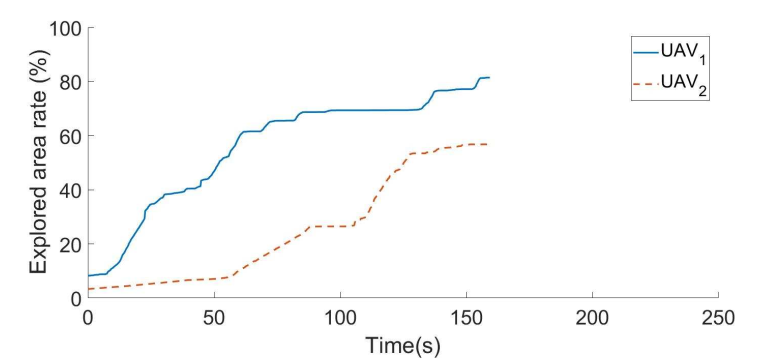
\includegraphics[width=\linewidth]{assets/3_18_b.png}
        \caption{{Hai UAV hợp tác.}}
        \label{fig:3.18b}
    \end{subfigure}
    \begin{subfigure}[H]{0.7\linewidth}
        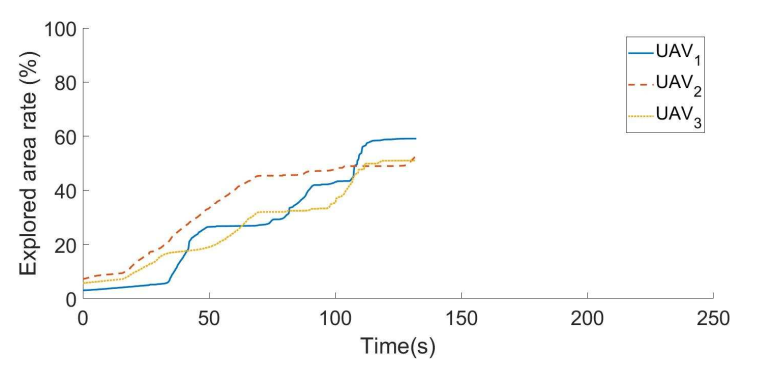
\includegraphics[width=\linewidth]{assets/3_18_c.png}
        \caption{{Ba UAV hợp tác.}}
        \label{fig:3.18c}
    \end{subfigure}
    \caption{Khám phá tỷ lệ không gian với một, hai và ba UAV.}
    \label{fig:3.18}
\end{figure}
\begin{figure}[H]
    \centering
    \begin{subfigure}[H]{0.7\linewidth}
        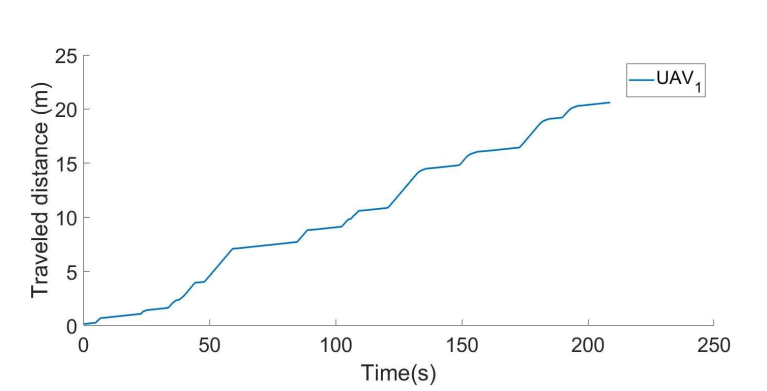
\includegraphics[width=\linewidth]{assets/3_20_a.png}
        \caption{{Một UAV.}}
        \label{fig:3.20a}
    \end{subfigure}
    \begin{subfigure}[H]{0.7\linewidth}
        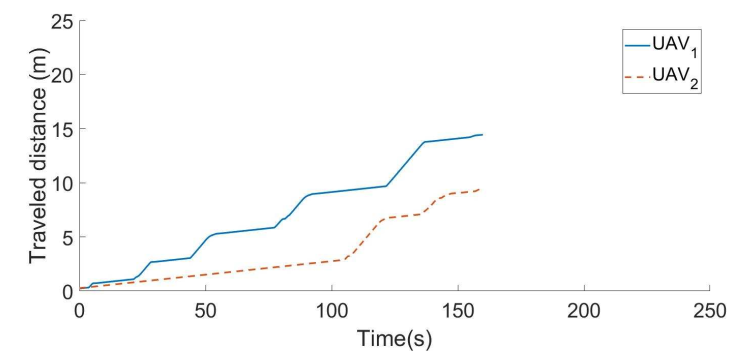
\includegraphics[width=\linewidth]{assets/3_20_b.png}
        \caption{{Hai UAV hợp tác.}}
        \label{fig:3.20b}
    \end{subfigure}
    \begin{subfigure}[H]{0.7\linewidth}
        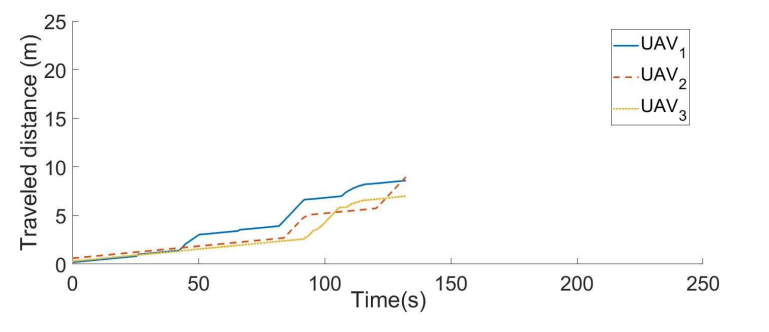
\includegraphics[width=\linewidth]{assets/3_20_c.png}
        \caption{{Ba UAV hợp tác.}}
        \label{fig:3.20c}
    \end{subfigure}
    \caption{Khoảng cách di chuyển của mỗi UAV với một, hai và ba UAV hợp tác.}
    \label{fig:3.20}
\end{figure}
Các khoảng cách được di chuyển bởi mỗi UAV bằng một, hai và ba UAV trong hạm đội được so sánh trong Hình \ref{fig:3.21}. Khoảng cách này giảm với số lượng UAV. Khoảng cách trung bình được di chuyển bởi mỗi UAV bị giảm bởi $55\%$ với 2 UAV và $62\%$ với 3 UAV. Lỗi của khoảng cách di chuyển được giảm nhẹ theo thứ tự từ một đến hai và ba UAV.
\begin{figure}[H]
    \centering
    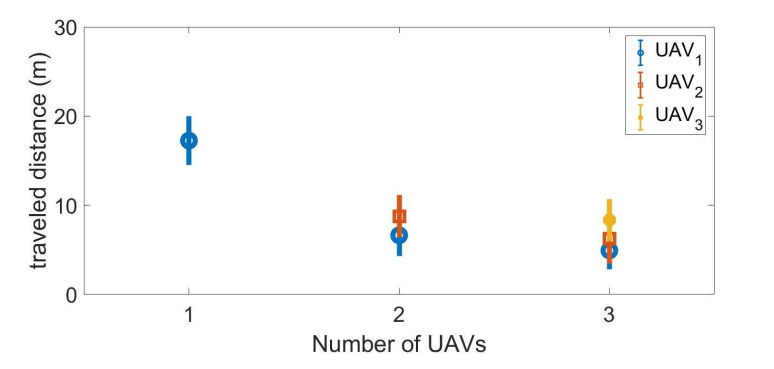
\includegraphics[scale=0.4]{assets/3_21.png}
    \caption{Đánh giá khoảng cách di chuyển được.}
    \label{fig:3.21}
\end{figure}
\subsubsection{Đánh giá thời gian khám phá}
Đối với đánh giá thời gian thăm dò, các lần chạy khác nhau đã được thực hiện bằng cách sử dụng 1, 2 và 3 UAV. Hình \ref{fig:3.22} cho thấy rằng trung bình của thời gian thăm dò giảm khi số lượng robot trong hạm đội tăng lên. Lỗi tính toán cũng giảm. Thời gian bị giảm đạt $25\%$ với 2 UAV và đạt $30\%$ với 3 UAV. Thời gian và khoảng cách thăm dò không được chia cho 2 hoặc 3 khi nhân với 2 hoặc 3 số lượng robot, tương ứng. Trong các mô phỏng này, vị trí ban đầu của robot là: $(1,0,0)$ cho một UAV; $(1,0,0)$ và $(1,-3,0)$ cho 2 UAV; và $(1,1,0)$, $(1,-1,0)$ và $(1,-3,0)$ cho 3 UAV.
\begin{figure}[H]
    \centering
    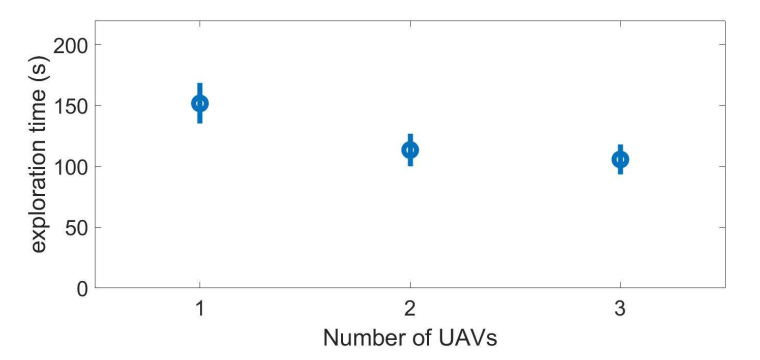
\includegraphics[scale=0.4]{assets/3_22.png}
    \caption{Thời gian thăm dò trung bình.}
    \label{fig:3.22}
\end{figure}
Các kết quả được trình bày trong Phần 4.2 được đánh giá mà không có bản địa hóa tương đối. Vì vậy, để có một kịch bản thực tế khó khăn hơn, chạy với thuật toán bản địa hóa tương đối đã được thực hiện để đánh giá các màn trình diễn hệ thống bằng SLAM.
\subsection{Nhiệm vụ khám phá bằng thuật toán bản địa hóa tương đối}
THướng tới một kịch bản thực tế hơn, cách tiếp cận ORB-SLAM2 (được giới thiệu trong Phần 5 của Chương 2) đã được triển khai để thực hiện bản địa hóa tương đối (Xem Hình \ref{fig:3.23}).
\begin{figure}[H]
    \centering
    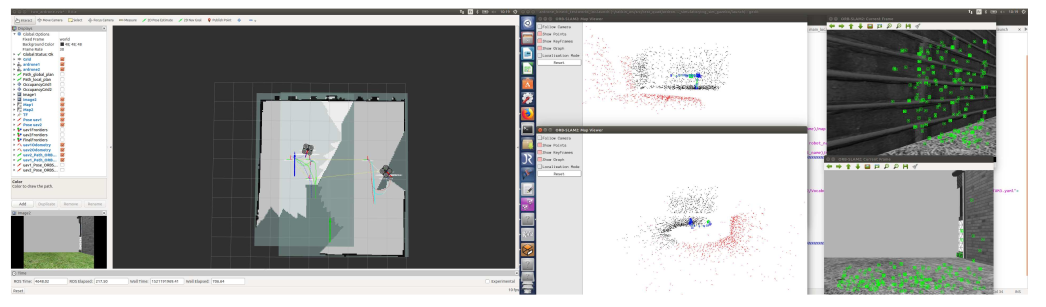
\includegraphics[scale=0.3]{assets/3_23.png}
    \caption{Hai điều hướng UAV bằng ORB-SLAM2.Hình ảnh Rviz (trái) hiển thị, đối với mỗi UAV, bản đồ lưới chiếm dụng 2D được xây dựng, quỹ đạo ước tính và sự thật tương ứng.Đám mây điểm (giữa) đại diện cho việc tái thiết thưa thớt môi trường được thực hiện bởi mỗi UAV.Và, các điểm đánh dấu màu xanh lá cây (phải) đại diện cho các tính năng được tính bằng mỗi UAV để thực hiện bản địa hóa.}
    \label{fig:3.23}
\end{figure}
Mỗi robot thực hiện SLAM nơi nó xây dựng bản đồ của nó trong khung tham chiếu cục bộ của nó $^WF_i$ , và ước tính tư thế tương đối của nó $\mathbf{p}_i$ bên trong nó. Sau đó, thiết bị thực hiện khám phá hợp tác bằng cách sử dụng một số thông tin cụ thể được trao đổi giữa các UAV. Tuy nhiên, những thông tin này phải nằm trong một hệ quy chiếu chung. Do đó, những thông tin như tư thế $\mathbf{p}_i$ và các điểm biên cương $\mathbf{f}_{i,j}$ nhất thiết phải biến thành khung tham chiếu toàn cầu $^0W$ trước khi được trao đổi.Vì thế \textit{leader} làm cho tất cả các tính toán cần thiết và gửi lại cho \textit{explorers} các mục tiêu trong $^0W$. Khi robot nhận được mục tiêu được giao, nó sẽ biến nó thành $^WF_i$ để lên kế hoạch cho một con đường đến nó.\\\\
Để thực hiện một phép chuyển đổi từ tham chiếu cục bộ $^WF_i$ đến toàn cầu một. $^0W$, Robot phải biết - ít nhất là - pose ban đầu của nó w.r.t. $^0W$. Như được giải thích trong Phần 5.2 của Chương 1, khung tham chiếu toàn cầu của môi trường được khởi tạo sao cho nó trùng với khung tham chiếu cục bộ của nhóm RST-\textit{leader} trong đội đó là UAV$_1$ Trong ví dụ được coi là phương trình \ref{eq:3.9}.
\begin{equation}\label{eq:3.9}
    ^0W\equiv ^WF_1,
\end{equation}
Sau đó, bằng cách phát hiện robot này bằng các thẻ được gắn trên đó, các robot khác có thể ước tính biến đổi tương ứng của chúng thành $^{F_j}\begin{bmatrix}\mathbf{R} & \mathbf{t}\end{bmatrix}_{F_1}, j \in [2..n_c]$. Để đánh giá mô phỏng, thông tin về biến đổi - được tính toán trong khi phát hiện thẻ - được giả định sẽ được biết đến. Hình \ref{fig:3.24} cho thấy sự phát triển tỷ lệ thăm dò trong nhiệm vụ thăm dò trong khi sử dụng ORB-SLAM2 làm phương pháp nội địa hóa tương đối.Thời gian truyền bá sử dụng ORB-SLAM2 bị giảm đi $43\%$ đối với 2 UAV thay vì 1 UAV.
\begin{figure}[H]
    \centering
    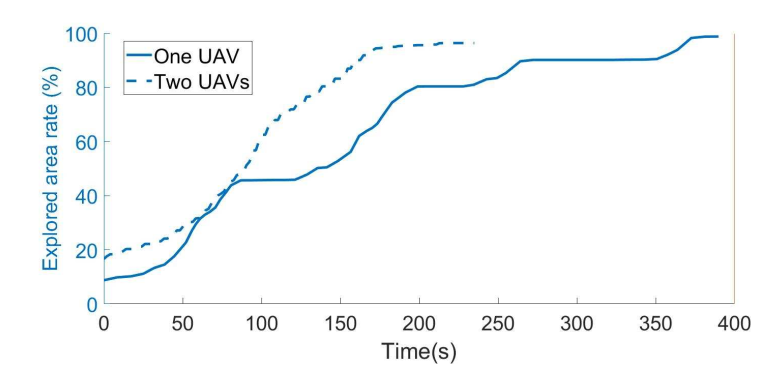
\includegraphics[scale=0.4]{assets/3_24.png}
    \caption{Khám phá sự tiến hóa tỷ lệ khu vực trong nhiệm vụ thăm dò với 1 và 2 UAV trong khi thực hiện ORB-SLAM2 bởi mỗi UAV.}
    \label{fig:3.24}
\end{figure}
Thời gian thăm dò khi sử dụng bản địa hóa tương đối (xem hình \ref{fig:3.24}) tương đối quan trọng so với việc khám phá mà không có slam (xem hình \ref{fig:3.18}) Vì vận tốc đã giảm đáng kể.
\section{Kết luận}
Trong chương này, chúng tôi đã trình bày một trạng thái của nhiệm vụ thăm dò đa robot bao gồm chiến lược được sử dụng để chỉ định robot cho mục tiêu và một chức năng tiện ích được áp dụng để ước tính sự quan tâm của việc tiếp cận nó. Sau đó, chúng tôi đã giới thiệu một chiến lược thăm dò dựa trên nhóm-\textit{leader} quyết định. Phân công robot - mục tiêu được thực hiện bằng cách sử dụng hàm tiện ích mới lạ. Hàm này tạo ra một giao dịch giao dịch giữa khám phá nhanh và nhận bản đồ lưới chi tiết, và cũng có tính đến khoảng cách của mỗi robot trong nhóm từ bộ mục tiêu chưa được khám phá. Ngoài ra, chúng tôi đề xuất để lên lịch để đạt được thông tin để truyền bá hiệu quả các UAV vào môi trường.Hơn nữa, chiến lược được thông qua trao đổi các điểm biên giới thay vì toàn bộ bản đồ địa phương.\\\\
Kết quả cho thấy chiến lược thăm dò hợp tác đề xuất giảm thiểu thời gian thăm dò toàn cầu theo $25\%$ cho 2 UAV và bởi $30\%$ cho 3 UAV, đồng thời giảm thiểu khoảng cách trung bình di chuyển của mỗi UAV bởi $55\%$ cho 2 UAV và bởi $62\%$ cho 3 UAV. Hơn nữa, chiến lược được đánh giá bằng thuật toán nội địa hóa tương đối nơi giảm thời gian thăm dò $43\%$ đối với 2 UAV thay vì 1 UAV.
%------------------CHAPTER 4------------------------------------------------%
\chapter{Giao tiếp giữa các robot}
\section{Giới thiệu}
Một chủ đề quan trọng trong các hệ thống nhiều robot là giao tiếp giữa các robot. Tính năng này được sử dụng để điều phối và chia sẻ thông tin cụ thể. Một đội có thể được triển khai trong một số nhiệm vụ trong các khu vực tương đối khác biệt và thù địch. Tuy nhiên, những môi trường này có thể không có cơ sở hạ tầng mạng sẵn có, ngoài các liên kết truyền thông không lý tưởng.\\\\
% This chapter highlights one of the most challenging points in MRS, which is the inter- robot communication. This problem can be addressed from different perspectives; but, we have chosen to study two sub-problems, which are: network typology, and network topology and strategy for MRS robustness.
Chương này nhấn mạnh một trong những điểm thách thức nhất trong MRS, đó là giao tiếp giữa các robot. Vấn đề này có thể được giải quyết từ các quan điểm khác nhau; nhưng, chúng tôi đã lựa chọn nghiên cứu hai vấn đề nhỏ, đó là: định dạng mạng, cấu trúc liên kết mạng và chiến lược cho sự mạnh mẽ của MRS.
\section{Phân loại mạng}
% The network is used to link between different entities and to establish possible communi- cation between them. Several network types exist and can be classified in different ways.
Mạng được sử dụng để liên kết giữa các thực thể khác nhau và để thiết lập giao tiếp có thể có giữa chúng. Một số loại mạng tồn tại và có thể được phân loại theo nhiều cách khác nhau.
\subsection{Chế độ cơ sở hạ tầng so với chế độ không có cơ sở hạ tầng}
Để quản lý cơ sở hạ tầng mạng, các chế độ hiện có có thể được phân loại thành hai loại chính \cite{bekmezci2013flying},\cite{hayat2015experimental}. Loại đầu tiên là chế độ cơ sở hạ tầng, có thể được gọi là chế độ Điểm truy cập (AP) và loại thứ hai là chế độ không có cơ sở hạ tầng, gọi là Ad Hoc mode (Xem Hình \ref{fig:4.1}). Trong chế độ AP, giao tiếp UAV-to-UAV được thực hiện thông qua cơ sở hạ tầng (AP, bộ định tuyến, v.v.), không giống như chế độ Ad Hoc trong đó các nút giao tiếp trực tiếp với nhau. Chế độ Ad Hoc còn được gọi là chế độ ngang hàng. Mạng Ad Hoc có thể phát triển thành một chế độ ngang hàng khác được gọi là mạng lưới bằng cách cho phép khả năng đa bước. Thật vậy, mạng Ad-Hoc không có bất kỳ khả năng cố hữu nào cho đa bước. Các nút giao tiếp với nhau khi chúng nằm trong phạm vi giao tiếp của nhau. Trong khi đó, trong mạng lưới, các nút có thể giao tiếp trực tiếp hoặc thông qua một hoặc nhiều nút trung gian.
\begin{figure}[H]
    \centering
    \includegraphics[scale=0.4]{assets/4_1.png}
    \caption{Chế độ hạ tầng (trái) và chế độ không có hạ tầng (phải).}
    \label{fig:4.1}
\end{figure}
\begin{table}[H]
    \centering
    \caption{Chế độ cơ sở hạ tầng so với chế độ không có cơ sở hạ tầng.}
    \label{tab:4.1}
    \begin{tabular}{|l|p{4.5cm}|p{4.5cm}|}\hline
                            & \textbf{Chế độ cơ sở hạ tầng}                 & \textbf{Chế độ không có cơ sở hạ tầng}
        \\\hline
        \textbf{Ưu điểm}    & Giao tiếp đáng tin cậy                        & Kết nối trực tiếp với nhau, dễ thiết lập, mạnh mẽ với lỗi nút, cho phép mở rộng và điều chỉnh trong cấu trúc liên kết mạng. \\\hline
        \textbf{Nhược điểm} & Phần cứng đắt, phức tạp, phạm vị bị hạn chế . & Thừa trong kết nối mạng, khó bảo trì.                                                                                       \\\hline
        \textbf{Tiêu chuẩn} & 802.11                                        & 802.11, 802.15, 802.16                                                                                                      \\\hline
    \end{tabular}
\end{table}
Ban đầu, robot phải thực hiện nhiệm vụ của chúng trong môi trường không có cơ sở hạ tầng mạng. Trên thực tế, chúng trao đổi thông tin khi chúng hoạt động như một bộ định tuyến và như một AP. Vì vậy, hệ thống MRS có thể được xem như một mạng Ad Hoc di động theo quan điểm giao tiếp.
\subsection{Phân loại mạng Ad Hoc}
Mạng Ad Hoc là mạng được sử dụng phổ biến để quản lý giao tiếp đa robot. Với mạng này, mỗi robot có thể di chuyển tự do và chuyển tiếp các gói tin đến và từ mỗi robot khác tùy thuộc vào phương thức phân phối dữ liệu \cite{bouachir2014conception}. Mạng này được đặc trưng bởi chất lượng dịch vụ phức tạp, trong đó giao thức định tuyến xác định đường đi tối ưu của thông tin có tính đến sự thay đổi thường xuyên của cấu trúc liên kết. Thêm vào đó, sẽ rẻ hơn nếu nhận ra loại mạng này thay vì các loại khác (vệ tinh, di động, v.v.).\\\\
Mạng Ad Hoc có thể được phân loại thành ba loại chính là Mobile Ah doc NETwork (MANET), Vehicle Ah doc NETwork (VANET) và Flying Ad hoc NETworks (FANET). Nói chung, đối với hệ thống đa UAV, mô hình FANET được sử dụng. Bảng \ref{tab:4.2} mô tả chi tiết mỗi đặc điểm của danh mục \cite{bekmezci2013flying}, \cite{maistrenko2016experimental}, phân tích dự đoán của chúng tôi.
\begin{table}[H]
    \centering
    \caption{So sánh giữa MANET, VANET, FANET và mô hình mạng của chúng tôi.}
    \label{tab:4.2}
    \begin{tabular}{|p{2.8cm}|p{1.5cm}|p{1.5cm}|p{1.8cm}|p{1.8cm}|}\hline
        \textbf{Đặc điểm}                                                 & \textbf{MANET}                                      & \textbf{VANET}                       & \textbf{FANET}                                                                                 & \textbf{Mô hình mạng của chúng tôi}
        \\\hline
        \textbf{Tính di động}                                             & Người ở một số địa hình nhất định                   & Phương tiện ở cao tốc                & Máy bay trong kế hoạch 3D                                                                      & 3D                                  \\\hline
        \textbf{Mức độ di động}                                           & $+$                                                 & $+$                                  & $++$                                                                                           & $++$                                \\\hline
        \textbf{Chế độ di động}                                           & Điểm cách ngẫu nhiên với hướng và tốc độ ngẫu nhiên & Có khả năng dự đoán cao trên đường   & Không được xác định trước (mô hình chuyển động ngẫu nhiên của UAV, mô hình dựa trên pheromone) & Có thể dự đoán                      \\\hline
        \textbf{Thay đổi cấu trúc liên kết}                               & $+$                                                 & $+$                                  & $++$                                                                                           & $++$                                \\\hline
        \textbf{Khoảng cách giữa các nút}                                 & $+$                                                 & $+$                                  & $++$                                                                                           & $+$                                 \\\hline
        \textbf{Mật độ nút}                                               & $++$                                                & $++$                                 & $+$                                                                                            & $+$                                 \\\hline
        \textbf{Mô hình truyền thanh}                                     & Sự hiện diện hiếm hoi của đường ngắm                & Sự hiện diện hiếm hoi của đường ngắm & Sự hiện diện thường xuyên của đường ngắm                                                       & Luôn có mặt của đường ngắm          \\\hline
        \textbf{Công suất tiêu thụ và công suất tính toán thời gian sống} & $+$                                                 & $+$                                  & $++$                                                                                           & $++$                                \\\hline
        \textbf{Tiêu chuẩn}                                               & IEEE 802.11, 802.15, 802.15.4, 802.16 and 802.20    & IEEE 802.11p                         & IEEE 802.11                                                                                    & ?                                   \\\hline
    \end{tabular}
\end{table}
So sánh cho thấy FANET là mạng gần nhất với kỳ vọng của mô hình của chúng tôi. Do đó, trong số các tiêu chuẩn hiện có cho loại mạng này, IEEE 802.11b và IEEE 802.11g cung cấp tốc độ dữ liệu cao và thường được sử dụng cho các hệ thống nhiều robot.
\subsection{Phân loại cấu trúc liên kết mạng}
Cấu trúc liên kết mạng xác định điểm đầu, điểm cuối và đường dẫn của thông tin trong mạng. Đã cho các điểm mục tiêu, cấu trúc liên kết xác định tất cả các con đường có thể để đạt được chúng.\\\\
Từ quan điểm phần mềm, mạng chủ yếu có thể được phân loại theo ba cấu trúc liên kết (Xem Hình \ref{fig:4.2}\footnote{Source: From user 1983 on Wikipedia. Licensed CC BY-SA}):
\begin{figure}[H]
    \centering
    \includegraphics[scale=0.4]{assets/4_2.png}
    \caption{Mạng tập trung (trái), phi tập trung (giữa) và mạng phân tán (phải).}
    \label{fig:4.2}
\end{figure}
\begin{itemize}
    \item Mạng tập trung: Đây là cấu trúc liên kết được sử dụng nhiều nhất \cite{morgenthaler2012uavnet}, \cite{forster2013collaborative}. Tất cả các nút - còn được gọi là các trạm - được kết nối với nhau thông qua một trung tâm tập trung. Đó là khi một nút cần gửi một thông tin đến một nút khác, dữ liệu nhất thiết phải đi qua nút trung tâm để được chuyển đến đích của nó. Nếu nút trung tâm không hoạt động hoặc không thể truy cập được, không có dữ liệu nào có thể được truyền đi, điều này làm cho cấu trúc liên kết này dễ bị lỗi nút.
    \item Mạng phân cấp: Cấu trúc liên kết này được coi là một tập hợp các mạng tập trung được kết nối với nhau \cite{konolige2003map}, \cite{brand2014stereo}. Một trung tâm chính được sử dụng cho mỗi nhóm nút nhỏ để gửi và nhận thông tin. Nếu một trung tâm bị lỗi, các nút liên quan trực tiếp đến nó sẽ không thể truy cập được.
    \item Mạng phân tán: Cấu trúc liên kết này chứa các nút được kết nối với nhau. Không giống như cấu trúc liên kết tập trung, một số đường dẫn có thể cùng đến một điểm. Ngoài ra, các nút không bị ảnh hưởng bởi lỗi của một nút. Điều này cho phép tăng khả năng sống sót và giảm hư hỏng cho mạng. Cấu trúc liên kết phân tán có tính hấp dẫn để đảm bảo mạng đáng tin cậy \cite{cunningham2010ddf}. Tuy nhiên, khá khó để tiếp cận và nhận ra trong thực tế, và mô phỏng không được phân phối đầy đủ \cite{waharte2009coordinated}, \cite{cameron2009collaborative}, \cite{scherer2015autonomous}. Điều này là do tất cả các quá trình xử lý và ra quyết định phải ở trên robot vốn đòi hỏi một bộ nhớ lớn và khả năng tính toán nặng.
\end{itemize}
\section{Cấu trúc mạng}
Cấu trúc của mạng thể hiện kiểu của nó cũng như các đặc điểm đã được giới thiệu.
\subsection{Công việc liên quan}
Giao tiếp MRS là một vấn đề quan trọng cần giải quyết trong cộng đồng robotics. Trong thập kỷ qua, sự tiến bộ vượt bậc trong công nghệ không dây và MRS đã tạo ra mối quan tâm ngày càng tăng đối với giao tiếp giữa các robot. Do đó, các phương pháp khác nhau đã được đề xuất.\\\\
Đối mặt với các tình huống thảm họa chẳng hạn như ở trong một nhà kho công nghiệp, tác giả của \cite{witkowski2008ad} đề xuất sử dụng mạng LAN không dây, Bluetooth và ZigBee để tạo thành mạng Ad-Hoc. Một số robot của hạm đội tạo thành cơ sở hạ tầng mạng để hỗ trợ giao tiếp.\\\\
Tác giả của \cite{morgenthaler2012uavnet} sử dụng hai tiêu chuẩn mạng để xây dựng một hệ thống đa UAV. Mạng lưới không dây IEEE 802.11s được xây dựng bằng cách sử dụng UAV mang các nút lưới được kết nối trực tiếp với thiết bị điện tử . Mỗi nút lưới này hoạt động như một AP để tạo thành IEEE 802.11g.\\\\
Phương pháp luận hỗ trợ giảm thiểu các liên kết không dây cho các phương tiện bay được nối mạng dựa trên Linux được trình bày trong \cite{kuschnig2012profiling.} Cách tiếp cận bao gồm hai tùy chọn để thu thập thông tin chất lượng liên kết và giám sát giao diện không dây 802.11.\\\\
Việc đánh giá tiêu chuẩn 802.11a được sử dụng giữa UAV và AP được thực hiện trong \cite{kuschnig2012profiling}. Kết quả cho thấy cường độ tín hiệu nhận (RSS) cho downlink giảm theo khoảng cách đến AP nhưng vẫn ở mức chấp nhận được cũng như thông lượng.\\\\
Biết rằng phổ ánh sáng nhìn thấy rộng hơn nhiều so với phổ Tần số vô tuyến, có vẻ thú vị khi sử dụng Visible Light Communication (VLC) dựa trên Light Emitting Diodes (LED). IEEE đã phát triển tiêu chuẩn 802.15.7 cho giao tiếp tầm ngắn sử dụng ánh sáng khả kiến. Tác giả của \cite{wang2014openvlc} giới thiệu giao tiếp hai chiều bằng Open VLC. Phần cứng giải pháp này cần bo mạch Beagle Bone Black (BBB) và bộ thu phát phông chữ sử dụng một đèn LED duy nhất để truyền và nhận. Giải pháp được triển khai trên trình điều khiển Linux giao tiếp trực tiếp với đèn LED front-end và ngăn xếp mạng Linux. Ý tưởng chính để sử dụng lại cùng một đèn LED cho cả tín hiệu Truyền (chế độ TX) và Tín hiệu ánh sáng nhận (chế độ RX) là khi một nút đang truyền dữ liệu, nút kia có thể mong đợi biểu tượng LOW của bit 0 và sử dụng thời gian này để chuyển chế độ của nó từ RX sang TX và truyền dữ liệu.\\\\
Zigbee - dựa trên IEEE 802.15.4 - là một giao thức ở mức cao, đặc biệt hữu ích cho phạm vi liên lạc ngắn và mức tiêu thụ thấp. Một số ứng dụng của UAV sử dụng mạng này \cite{asadpour2014routing}. Giao tiếp có thể được thực hiện dưới ba dải tần tùy thuộc vào loại chipset: 868MHz cho tốc độ bit 20 kbps, 915MHz cho 40 kbps và 2,4 GHz cho 250 kbps.\\\\
Tác giả trong \cite{vidal2015multi} thông qua các nhóm có quy mô khác nhau bao gồm các UAV chiến thuật và UAV di chuyển trong các khu vực địa lý được phân định. Các kỹ thuật ảo hóa được sử dụng để điều chỉnh việc nâng cấp bất kỳ chức năng nào, cho phép khả thi trong các dịch vụ không đồng nhất.\\\\
Trong một nhiệm vụ tìm kiếm và cứu hộ, ví dụ, các tác giả trong \cite{scherer2015autonomous} đề xuất phát trực tuyến thời gian thực giữa các UAV trên một khoảng cách lớn. Nhiệm vụ được chia thành 5 giai đoạn chính: Lập kế hoạch trước để xác định các con đường tốt nhất trong khu vực tìm kiếm cho phép giảm thời gian của nhiệm vụ sau đó tìm kiếm chỉ theo các điểm chỉ dẫn trước; việc phát hiện mục tiêu và gửi các kế hoạch mới cho những người khác, tiếp theo là định vị lại bằng cách thiết lập một liên kết đa bước để đánh giá tình hình bởi trạm gốc và cuối cùng là phát trực tuyến video.\\\\
Đa UAV cần hệ thống truyền dẫn phức tạp để đảm bảo tính khả thi khi di chuyển trong không gian ba chiều . Trong \cite{scherer2015autonomous}, một ăng ten đẳng hướng đa hướng được bố trí trên trạm gốc và trên tất cả các UAV không đồng nhất được triển khai. Để trao đổi dữ liệu, công nghệ lưới chuẩn IEEE 802.11s được sử dụng.\\\\
Các tác giả trong \cite{hayat2015experimental} so sánh hiệu suất giữa IEEE 802.11n tiêu chuẩn và IEEE 802.11ac trong mạng đa bước. Các mạng thứ đã được thử nghiệm trong môi trường trong nhà và ngoài trời, và ở hai chế độ, chế độ điểm truy cập (AP) / chế độ cơ sở hạ tầng và chế độ lưới liên quan đến thông lượng và công bằng. Trong các thử nghiệm trong nhà, đối với chế độ cơ sở hạ tầng, 802.11ac cho thấy hiệu suất được cải thiện trong cả thông lượng TCP và UDP, và mất gói đối với đường truyền UDP. Trong các thí nghiệm ngoài trời, đối với chế độ cơ sở hạ tầng, thông lượng của 802.11n cao hơn gấp ba lần so với 802.11a, tuy nhiên, chất lượng liên kết giảm mạnh hơn. Đối với chế độ lưới, 802.11n đạt được thông lượng cao hơn ở phạm vi gần nhưng giảm nhanh hơn ngay khi tốc độ ngày cao hơn và phạm vi dài hơn. Thông lượng được ghi lại cho mạng lưới thấp hơn chế độ cơ sở hạ tầng do thời gian truyền liên gói dài hơn.\\\\
Đối mặt với các vấn đề về bảo trì kết nối, tránh va chạm, tính chắc chắn khi gặp lỗi và cải thiện vùng phủ sóng, các tác giả trong \cite{ghedini2018toward} đề xuất một mô hình mới cung cấp nhiều cấu trúc liên kết mạng tốt hơn.\\\\
Trong \cite{harms2017development}, một lớp giao tiếp mới được đề xuất để đối phó với các mạng yêu cầu băng thông cao. Vì vậy, một số cơ chế được sử dụng để gửi thông báo, nén dữ liệu hoặc phản ứng với các tình huống bất ngờ.\\\\
Bảng \ref{tab:4.3} liệt kê một số tiêu chuẩn được sử dụng trong hệ thống nhiều robot. Đối với mỗi tiêu chuẩn, chúng tôi trình bày chi tiết lớp liên quan trong mô hình OSI, các đặc điểm của nó, kết quả hoạt động cũng như phần cứng và phần mềm được sử dụng cho các thí nghiệm.
\begin{landscape}
    \begin{table}[H]
        \centering
        \caption{Ví dụ về một số tiêu chuẩn được sử dụng trong MRS.}
        \label{tab:4.3}
        \begin{tabular}{|p{1.5cm}|p{1.7cm}|p{1.3cm}|p{2.9cm}|p{2.7cm}|p{2.3cm}|p{2cm}|}\hline
            \textbf{Bài báo}                          & \textbf{Tiêu chuẩn}          & \textbf{Lớp}   & \textbf{Đặc trưng}                                                            & \textbf{Hiệu năng}                                                                       & \textbf{Phần cứng}                                                              & \textbf{Phần mềm}
            \\\hline
            [Scherer et al., 2015]                    & IEEE 802.11s mesh technology & Lớp Network    & Tương thích với chế độ lưới và chế độ AP                                      & Range: 100m, communication delay: 5ms, Throughput: 10-20Mbit/s                           & Heterogeneous UAVs + laptop BS + wifi module                                    & Middleware Robot Operating System ROS       \\\hline
            \multirow{2}{1.5cm}{[Hayat et al., 2015]} & IEEE 802.11n                 & Lớp PHY và MAC & Thông lượng cao ở cả hai chế độ (AP và lưới), mức độ công bằng chấp nhận được & Outdoor + mesh mode + single hop; Range: 500m; TCP throughput: 35Mbit/s (50m); FB: 40Mhz & Two Pelican UAVs + laptop BS + Compex WLE300NX 802.11abgn mini PCIe modules     & Ubuntu Linux Kernel 3.2. with ath9k driver  \\\cline{2-7}
                                                      & IEEE 802.11ac                & Lớp PHY và MAC & Không hỗ trợ chế độ lưới                                                      & Outdoor + mesh mode + single hop; Range: 500m; TCP throughput: 10Mbit/s (50m); FB: 80Mhz & Two Pelican UAVs + laptop BS + Compex WLE900N518 802.11ac 5Ghz miniPCIe modules & Ubuntu Linux Kernel 3.2. with ath10k driver \\\hline
        \end{tabular}
    \end{table}
\end{landscape}
\begin{landscape}
    \begin{table}[H]
        \centering
        \begin{tabular}{|p{1.5cm}|p{1.7cm}|p{1.3cm}|p{2.9cm}|p{2.7cm}|p{2.3cm}|p{2cm}|}\hline
            [Kuschnig et al., 2012] & IEEE 802.11a           & Lớp PHY và MAC & RSS và thông lượng giảm dần theo khoảng cách nhưng vẫn ở mức chấp nhận được        & Outdoor over compus 150m*150m; Range: 10m; Throughput: 54Mbit/s (theo) and 27Mbit/s (prac); FB: 5Ghz                        & AP: Netgear WNDR3700 + Atheros AR9280 based wireless cards + UAV with Intel Atom Processor + SparkLAN WPEA110N wireless card + antenna WIMO 18720.11 for UAV and AP & Linux-based OpenWRT Backfire 10.03.1RC5 \\\hline
            [Asadpour et al., 2014] & IEEE 802.11n multi hop & Lớp PHY và MAC & Thời gian hội tụ lâu và chi phí định tuyến cao (với giao thức BATMAN cho Lớp mạng) & In-flight experiment; Throughput for 200m: 5.95Mbit/s; Convergence time (20-100m): 28s; Routing overhead (20-100m): 10msg/s & Two Arducopter + GB + WLAN IEEE 802.11n + XBEE-PRO                                                                                                                  &                                         \\\hline
        \end{tabular}
    \end{table}
\end{landscape}
\begin{landscape}
    \begin{table}[H]
        \centering
        \begin{tabular}{|p{1.5cm}|p{1.7cm}|p{1.3cm}|p{2.9cm}|p{2.7cm}|p{2.3cm}|p{2cm}|}\hline
            [Morgen- thaler et al., 2012] & IEEE 802.11s mesh nodes for UAV to UAV and IEEE 802.11g for UAV to AP & Lớp Network    & Trong một bước nhảy, các UAV đạt được thông lượng cao hơn các UAV trên mặt đất. Các kết quả này được thực hiện với chế độ định vị dựa trên vị trí thấp hơn so với chế độ định vị cường độ tín hiệu. Những màn trình diễn này cao hơn so với multi-hop. & Single hop (1UAV altitude 3-5m and AP-AP = 75m) in location positioning mode; TCP throughput = 6.5Mbit/s + in signal strength positioning mode: TCP throughput = 8.1Mbit/s & One UAVNet quadcopters Professional Mesh OM1P + two notebooks & Linux 2.6.37.6 Kernel generated by ADAM (embedded Linux distribution) + driver ath5k \\\hline
            [Muzaffar and Yanmaz, 2014]   & IEEE 802.11ab                                                         & Lớp PHY và MAC & Thông lượng giảm khi số lượng nút tăng lên                                                                                                                                                                                                             & Range: up to $1000m \times 1000m \times 50m$; Throughput: 54Mbit/s (prac); FB: 5Ghz                                                                                        & Simulation: UAVs + Groung Station                             & Omnet++                                                                              \\\hline
        \end{tabular}
    \end{table}
\end{landscape}
\begin{landscape}
    \begin{table}[H]
        \centering
        \begin{tabular}{|p{1.5cm}|p{1.7cm}|p{1.3cm}|p{2.9cm}|p{2.7cm}|p{2.3cm}|p{2cm}|}\hline
            [Wang et al., 2014] & IEEE 802.15.7 & Lớp PHY và MAC & Truyền hai chiều, kết hợp lọc và khôi phục lỗi thời gian có thể tăng phạm vi liên lạc và độ ổn định & \textit{One hop}: throughput: 1.6kb/s, packet loss ratio $5\%$; \textit{Two hop:} throughput 0.65kb/s, packet loss ratio $15\%$ & Embedded BBB board + LED front end & Linux Kernel 3.8.13 \\\hline
        \end{tabular}
    \end{table}
\end{landscape}
\subsection{Các tiêu chuẩn và giao thức mạng}
Kể từ khi trao đổi thông tin là cần thiết để phối hợp, mạng được sử dụng cho truyền thông đa UAV phải đảm bảo rằng thông tin lưu thông đúng cách trong các nút.Do đó, chúng ta phải vượt qua một số vấn đề như:
\begin{itemize}
    \item Lỗi nút: Khi liên kết bị hỏng hoặc bị lỗi, mạng phải tìm đường dẫn để đến nút.
    \item Thay đổi cấu trúc liên kết: Các nút di chuyển trong môi trường và tạo ra những thay đổi trong cấu trúc liên kết mà mạng phải đối phó nhanh chóng.
    \item Băng thông liên lạc: UAV sở hữu một số thông tin nhất định để trao đổi với các thông tin khác và cần một số băng thông hỗ trợ trao đổi dữ liệu.
\end{itemize}
Có tính đến các vấn đề được trích dẫn ở trên và để đảm bảo tích hợp tốt giữa SLAM trực quan và giao tiếp, mạng lưới không dây phân phối và hợp tác dường như là kiểu chữ mạng đầy đủ nhất. Nó cho phép giới thiệu những lợi thế sau:
\begin{itemize}
    \item Cải thiện độ tin cậy của mạng vì mạng không có cơ sở hạ tầng yêu cầu một số đường dẫn, để thông tin có thể đến đích ngay cả khi chỉ có một liên kết bị hỏng.
    \item Cho phép khả năng mở rộng của mạng bằng cách thích ứng nhanh với các thay đổi cấu trúc liên kết.
    \item Cho phép triển khai nhanh chóng với chi phí back-haul.
    \item Cung cấp bảo hiểm dễ dàng trong các khu vực có quyền truy cập khó khăn.
    \item Tiết kiệm tuổi thọ pin do tiêu thụ điện năng thấp hơn.
    \item Cho phép đối mặt với một số lượng lớn các UAV trong một hạm đội.
\end{itemize}
Trong số các tiêu chuẩn mạng lưới hiện có, sửa đổi 802.11, liên quan đến lớp Mac, thú vị cho các ứng dụng MRS. Nó là một mạng thiết lập dịch vụ mở rộng hỗ trợ giao tiếp phát sóng, phát đa hướng và unicast.Nó chứa giao thức Hybrid Wireless Mesh Protocol (HWMP) làm giao thức định tuyến mặc định.HWMP là một giao thức định tuyến lai lấy cảm hứng từ AODV (Ad-hoc On-demand Distance Vector: một phần theo yêu cầu và phần phản ứng) và giao thức dựa trên cây (một phần chủ động). Qua đó, nó chứa các ưu điểm của giao thức phản ứng vì nó chuẩn bị bảng định tuyến khi các nút thay đổi vị trí của chúng và do đó cung cấp đường dẫn an toàn hơn. Mặt khác, nó chứa những ưu điểm của giao thức chủ động vì bảng định tuyến đã sẵn sàng cho phép tiết kiệm thời gian khi cần thiết. Ngoài giao thức định tuyến mặc định HWMP, mạng lưới 802.11S hỗ trợ các giao thức khác như Optimized Link State Routing (OLSR), Better Approach to Mobile Ad hoc Networking (BATMAN), Wireless Distribution System (WDS), Open Shortest Path First (OSPF) và BABEL. Theo \cite{wang2010experimental}, BATMAN đã chứng minh khả năng tốt hơn HWMP và OLSR. Do đó, các thí nghiệm sử dụng HWMP và BATMAN đã được thực hiện để chỉ ra dữ liệu đã lưu.
\paragraph{Định nghĩa giao thức BATMAN}
Giao thức BATMAN\footnote{Nguồn: \url{https://www.open-mesh.org/projects/open-mesh/wiki}} là một giao thức định tuyến chủ động lấy cảm hứng từ AODV và OLSR. Nó được hỗ trợ bởi các mạng lưới multi-hop Ad Hoc. Nó sử dụng các phương pháp khác nhau để định tuyến nút chọn bằng cách gửi OriGinator Messages (OGM) cho hàng xóm với thông tin nút đến next hop và đích đến tiếp theo vì các quyết định định tuyến được phân phối trên các nút. Trong giao thức này, mỗi nút quyết định cho next hop và không cho toàn bộ tuyến đường để các nút không sử dụng hoặc thậm chí biết cấu trúc liên kết của mạng.Trong trường hợp phát hiện các nút khác, giao thức BATMAN sẽ dẫn con đường tốt nhất cho họ. Nó cũng theo dõi các nút mới và thông báo cho hàng xóm về sự tồn tại của họ.
\subsection{Kết quả và thảo luận}
Để đánh giá hệ thống nối mạng bằng cách sử dụng giao thức BATMAN\footnote{The BATMAN-adv version used for the testbed is available since 2013}, Chúng tôi sử dụng các nút không đồng nhất gồm ba máy tính xách tay: 2.40GHz dual core Linux machine, 2.27GHz i3 Linux machine, 2.50GHz i5 Linux machine and a Parrot AR-Drone 2.0 (Xem Hình \ref{fig:4.3}).
\begin{figure}[H]
    \centering
    \includegraphics[scale=0.3]{assets/4_3.png}
    \caption{Mạng lưới minh họa giữa ba máy tính xách tay và một máy bay không người lái.}
    \label{fig:4.3}
\end{figure}
Chúng tôi mô phỏng việc phát sóng dữ liệu giữa các nút trong cả mạng Ad Hoc và lưới với giao thức BATMAN để nhấn mạnh dữ liệu đã lưu. Máy bay không người lái đã được điều khiển từ máy tính xách tay bằng cách sử dụng biên dịch chéo. Đầu tiên, chúng tôi thực hiện một mạng Ad Hoc giữa các điểm cuối và phát dữ liệu từ nút A đến nút B, C và D trong mạng. Sau đó, chúng tôi phát sóng - trong cùng điều kiện - từ nút A đến B, C và D với giao thức mạng lưới BATMAN. Kết quả như Hình \ref{fig:4.4} cho thấy thông lượng đạt được trung bình 0.4 Mbits/s; trong khi đó, thông lượng được đánh giá trong mạng lưới với giao thức BATMAN, đạt mức trung bình 0.65 MBits/s. Giao thức mạng lưới BATMAN cải thiện 1,5 lần thông lượng của mạng so với mạng Ad Hoc cơ bản.
\begin{figure}[H]
    \centering
    \includegraphics[scale=0.4]{assets/4_4.png}
    \caption{Phát sóng thông lượng được phát sóng trong giao thức mạng Ad Hoc và BATMAN.}
    \label{fig:4.4}
\end{figure}
\section{Cấu trúc liên kết và chiến lược mạng cho MRS robustness}
Cấu trúc liên kết của mạng xác định các thuộc tính hình học của các nút (ở đây là robot). Chiến lược đề xuất trong công việc này thể hiện hành vi được áp dụng để đối mặt với các tình huống quan trọng và để đạt được MRS robustness.
\subsection{Công việc liên quan}
Thách thức trong giao tiếp MRS là duy trì mạng đáng tin cậy trong nhiệm vụ làm cho robot có thể thực hiện hợp tác thăm dò \cite{rooker2007multi}, \cite{gupta2015survey}. Chiến lược được sử dụng để thăm dò ảnh hưởng đến việc trao đổi dữ liệu giữa các robot bao gồm loại, điểm đến và tần số.\\\\
Thông tin trao đổi giữa robot và một máy chủ có thể là khung hình chính và điểm bản đồ \cite{schmuck2017multi}, hoặc chỉ các tính năng của các khung hình chính được chọn và ước tính relative-pose giữa robot và trạm mặt đất \cite{forster2013collaborative}. Nhưng chủ yếu, robot trao đổi các bản sao địa phương của họ về bản đồ và các pose của họ \cite{fox2006distributed}, \cite{bresson2015general}, \cite{schuster2015multi}.\\\\
Lượng dữ liệu trao đổi có thể tăng nhanh về kích thước, có thể gây tắc nghẽn mạng và mất dữ liệu. Để giảm yêu cầu băng thông, các tác giả của \cite{mohanarajah2015cloud} Đề xuất chỉ gửi các key-frames và các vị trí key-frames được cập nhật. Ngoài ra, các tác giả trong \cite{cunningham2010ddf} đề xuất một cách tiếp cận Decentralized Data Fusion-Smoothing And Mapping (DDF-SAM), trong trường hợp mỗi robot tuyên truyền tới  các robot khác, đồ thị cục bộ cô đọng của nó để đạt được khả năng mở rộng và khả năng chống lại lỗi nút.\\\\
Hầu hết các công việc liên quan đến giải quyết các vấn đề giao tiếp trong khi giả định một mạng lưới lý tưởng hoặc mục đích giữ cho các thành viên trong phạm vi của nhau để tập trung sự chú ý vào các vấn đề quan trọng hơn \cite{scherer2015autonomous}, \cite{burgard2005coordinated}.\\\\
Xem xét tổn thất giao tiếp và/hoặc băng thông hạn chế giúp ngăn ngừa thất bại nhiệm vụ và để đảm bảo một kịch bản thực tế hơn. Thật vậy, trong các kịch bản thực tế, nhiều vấn đề có thể phát sinh như có khoảng cách giữa các robot vượt quá phạm vi giao tiếp, mất thông tin chính trong một liên kết giao tiếp bị hỏng, tốn thời gian trong việc gửi thông tin do băng thông hạn chế, v.v.. Chiến lược thăm dò phải tính đến các vấn đề được đề cập để tránh nhiệm vụ thất bại trong kịch bản thế giới thực. Một số công việc đã bắt đầu giải quyết vấn đề thăm dò trong khi xem xét các giới hạn giao tiếp \cite{couceiro2014darwinian}, \cite{schmuck2017multi}.\\\\
Trong \cite{dai2018quality}, mục đích là để cảm nhận một môi trường phức tạp về hình học bằng cách gán các mục tiêu cho robot khi độ phân giải không gian và thời gian là hợp lý. Cách tiếp cận này sử dụng thuật toán lập kế hoạch đường dẫn năng lượng min-max tuân theo thời hạn.\\\\
Trong công việc này, chúng tôi lựa chọn để cho UAV trao đổi với nhau chỉ qua các điểm biên giới, robot đặt ra và các mục tiêu được chỉ định. Trao đổi này xảy ra ở mỗi lần lặp trong khi xem xét vai trò của UAV, được điều chỉnh theo cấu trúc liên kết mạng.Thích ứng này cũng cho phép đối phó với những hạn chế giao tiếp.
\subsection{Phương pháp giao tiếp giữa các robot}
Tương tác giữa các thành viên của đội tàu rất quan trọng đặc biệt là trong các nhiệm vụ thăm dò để ngăn chặn UAV khám phá các khu vực giống nhau và cho phép họ hợp tác khám phá các khu vực chưa biết nhanh hơn và một cách tối ưu hóa. Tuy nhiên, liên lạc giữa các UAV là một vấn đề đầy thách thức đòi hỏi phải trả lời một số câu hỏi thực tế: Loại nút dữ liệu nào phải trao đổi? Làm thế nào để dữ liệu nên được chia sẻ một cách thường xuyên? Chúng ta có nên xem xét một trao đổi dữ liệu nhiều hop? Nếu vậy, làm thế nào để xác định điểm cuối của trao đổi dữ liệu? Làm thế nào để đối phó với những hạn chế giao tiếp? Những câu hỏi này được giải quyết trong các tiểu mục sau.
\subsubsection{Tương tác đa UAV và trao đổi dữ liệu}
Trong chiến lược hợp tác thăm dò đề xuất, điểm biên giới địa phương $\mathbf{f}_{i,j} \in \mathcal{F}$, pose hiện tại $\mathbf{p}_i$ , và điểm mục tiêu hiện tại $\mathbf{t}_m$ được trao đổi thay vì toàn bộ bản sao của bản đồ địa phương. Điều này dự kiến sẽ tạo ra sự giảm đáng kể khối lượng dữ liệu trao đổi, và do đó, giảm tiêu thụ bộ nhớ. Sơ đồ trình tự\footnote{This diagram uses Unified Modeling Language's sequence diagram notation.} trong Hình \ref{fig:4.5} thể hiện chi tiết (thời gian và thông tin) các tin nhắn trao đổi giữa hai UAV. UAV$_i$ , với $i \in [1..n_c]$ và UAV$_j$ với $j \in [2..n_c] (i<j)$ là các robot trong cụm $\mathcal{C}$. Họ chuyển tiếp ID tương ứng và poses hiện tại của họ $\mathbf{p}_i$ và $\mathbf{p}_j$. Từ $i < j$, \textit{explorer} UAV$_j$ gửi đến \textit{leader} UAV$_i$ điểm biên cục bộ của nó $\mathbf{f}_{j,k}$ trong bước xử lý biên giới (FP).
\begin{figure}[H]
    \centering
    \includegraphics[scale=0.5]{assets/4_5.png}
    \caption{Luồng dữ liệu giữa hai robot. FP và GA đứng tương ứng, để xử lý biên giới và phân công mục tiêu.}
    \label{fig:4.5}
\end{figure}
Sau đó, \textit{leader} thực hiện quy trình phân công mục tiêu (GA) và gửi lại UAV$_j$ điểm mục tiêu đã chọn $\mathbf{t}_m$ . Ví dụ được trích dẫn đại diện cho hai UAV trong cụm $\mathcal{C}$. Trong trường hợp nhiều UAV trong $\mathcal{C}$, các chuỗi tương tự sẽ được thực hiện giữa một \textit{leader} và nhiều \textit{explorers}.
\subsubsection{Chiến lược exploration để đối mặt với mất giao tiếp}
Trong hệ thống đề xuất, xem xét các hạn chế truyền thông rất quan trọng để đảm bảo tính liên tục của nhiệm vụ. Trong trường hợp mất liên lạc với \textit{leader} do thất bại giao tiếp hoặc UAV bị kẹt, một \textit{leader} khác được tự chọn trong lần lặp tiếp theo để nhiệm vụ có thể tiếp tục. Trong Hình \ref{fig:4.6}, tại $t=t_n$ , hạm đội bao gồm một cụm nơi UAV có thể giao tiếp với nhau. Một \textit{leader} xử lý các quyết định cho người khác. Tại $t=t_{n+1}$, liên kết truyền thông thất bại giữa UAV$_3$ và UAV$_4$. Hạm đội được chia thành hai cụm với mỗi một \textit{leader}.
\paragraph{Trường hợp đặc biệt}
Trong trường hợp mất liên lạc với \textit{leader} và một \textit{leader} đã được chọn, \textit{explorers} để một bộ đếm thời gian $\tau$ hết hạn trong khi chờ chuyển nhiệm mục tiêu. Nếu không có mục tiêu được nhận, \textit{explorer} chọn mục tiêu riêng của nó theo thông tin địa phương.\\\\
Sử dụng chiến lược này, miễn là - ít nhất - một UAV tồn tại trong hạm đội, nhiệm vụ sẽ tiếp tục cho đến khi tất cả các môi trường giới hạn được khám phá (không có điểm biên giới ứng cử viên nào còn lại).
\subsubsection{Thảo luận chiến lược trao đổi dữ liệu}
Trong chiến lược được đề xuất, trao đổi dòng dữ liệu được lặp lại tại mỗi lần lặp trong khi có tính đến các thay đổi cấu trúc liên kết mạng để xác định các cụm. Các điểm bắt đầu và điểm cuối được xác định theo các vai trò này. Vai trò của UAV cũng chỉ định loại dữ liệu trao đổi. Ngoài việc trao đổi pose hiện tại $\mathbf{p}_i$ và $id$ số $i$, nếu UAV$_i$ là một \textit{explorer}, nó sẽ thụ động chia sẻ thông tin về chính nó và môi trường xung quanh với \textit{leader} (điểm biên giới $\mathbf{f}_{i,j} \in \mathcal{F}$); khác, vai trò của nó sẽ là gửi mục tiêu để truy cập đến \textit{explorers} (điểm mục tiêu $\mathbf{t}_k \in \mathcal{G}$).
\begin{figure}[H]
    \centering
    \includegraphics[scale=0.4]{assets/4_6.png}
    \caption{Sự tiến hóa vai trò trong phạm vi giao tiếp hạn chế.}
    \label{fig:4.6}
\end{figure}
Chiến lược đề xuất đảm bảo tính một nhiệm vụ liên tục trong trường hợp mất liên lạc. Tuy nhiên, UAV có thể khám phá các khu vực đã được các nút khác khám phá, vì không có bản đồ địa phương nào được trao đổi cũng không được hợp nhất để theo dõi các khu vực truy cập. Do đó, trong trường hợp mất truyền thông, thành tựu được ưa chuộng đối với việc giảm thiểu tiêu thụ tài nguyên, chẳng hạn như thời gian và pin.
\subsection{Kết quả và thảo luận}
Vì UAV được trang bị thẻ không dây IEEE 802.11b,g, chúng tôi thiết lập một mạng lưới cơ sở hạ tầng trong tập hợp các robot để định lượng trao đổi dữ liệu giữa các thành viên của đội tàu, cũng như, để xác định hiệu suất của mạng robot. Thực hiện chạy với 2 và 3 UAV (Xem Hình \ref{fig:4.7}). Mạng được bao gồm hai thiết bị là một 2.60GHz i7 Linux machines và một 2.50GHz i7 Linux machine. Số lượng robot được sử dụng để đánh giá được giới hạn ở 3, tuy nhiên, kiến trúc hệ thống được đề xuất không bị hạn chế với một số robot cố định.
\begin{figure}[H]
    \centering
    \begin{subfigure}[H]{0.7\linewidth}
        \includegraphics[width=\linewidth]{assets/4_7_a.png}
        \caption{{Hai UAV (Laptops)}}
        \label{fig:4.7a}
    \end{subfigure}
    \begin{subfigure}[H]{0.7\linewidth}
        \includegraphics[width=\linewidth]{assets/4_7_b.png}
        \caption{{Ba UAV (Laptops).}}
        \label{fig:4.7b}
    \end{subfigure}
    \caption{Minh họa mạng Ad Hoc trong nhiệm vụ thăm dò.}
    \label{fig:4.7}
\end{figure}
\subsubsection{Cài đặt mạng: Từ một đến nhiều máy}
Khi chạy nhiều UAV trên một máy duy nhất (như trong các mô phỏng trước đó trong Chương 3), một ROS master có trách nhiệm quản lý giao tiếp intra và inter-processes bằng cách sử dụng publisher/subscriber. Trong trường hợp nhiều máy, hai cấu hình có thể:
\begin{itemize}
    \item Một ROS core cho nhiều máy (Xem Hình \ref{fig:4.8a}): Ngay cả với nhiều UAV trên các máy khác nhau, một ROS master/core có thể được áp dụng bằng cách chỉ định máy chạy ROS core. Trong trường hợp này, SoS sẽ quản lý giao tiếp inter-processes theo cùng một cách như thể chúng nằm trên cùng một máy. Ngoại lệ là giao tiếp trong thế giới thực được sử dụng thay vì bộ nhớ dùng chung để chạy nhiều UAV trên một máy.
    \item Nhiều ROS cores cho nhiều máy (Xem Hình \ref{fig:4.8b}): Khi chạy các ROS core khác nhau trên các máy khác nhau, mỗi chiếc UAV quản lý chủ của chính nó.Trong hệ thống đa lõi này - còn được gọi là hệ thống đa chủ -, đồng bộ hóa trong số các master này cần phải được thực hiện.
\end{itemize}
Tuy nhiên, đối với cả hai trường hợp, môi trường ảo sẽ được khám phá trong \textit{Gazebo} phải giống nhau để UAV khám phá cùng một môi trường cùng một lúc. Cụ thể, điều này có nghĩa là IP client của \textit{Gazebo} phải phù hợp với IP server của máy chạy \textit{Gazebo} thế giới bằng cách thiết lập $\textit{GAZEBO\_MASTER\_URI}$.\\\\
Khi chạy một ROS core cho nhiều UAV, một mạng đáng tin cậy là cần thiết, quá trình  ROS khác sẽ không hoạt động đúng khi kết nối mạng không ổn định. Ngoài ra, chạy hệ thống multi-master là thực tế hơn bởi vì trong thế giới thực, mỗi UAV phải là thuộc về chức năng, độc lập và hợp tác để đạt được các mục tiêu nhiệm vụ, trong công việc này, việc khám phá một môi trường không xác định. Một hệ thống multi-master đại diện cho cấu hình hệ thống phân tán, có những ưu điểm khác nhau như khả năng mở rộng cho khả năng chịu lỗi.
\begin{figure}[H]
    \centering
    \begin{subfigure}[H]{0.4\linewidth}
        \includegraphics[width=\linewidth]{assets/4_8_a.png}
        \caption{{Một ROS core cho nhiều máy.}}
        \label{fig:4.8a}
    \end{subfigure}
    \begin{subfigure}[H]{0.4\linewidth}
        \includegraphics[width=\linewidth]{assets/4_8_b.png}
        \caption{{Nhiều ROS cores cho nhiều máy.}}
        \label{fig:4.8b}
    \end{subfigure}
    \caption{{Hai cấu hình ROS trong trường hợp nhiều máy. Ảnh từ \cite{andre2014coordinated}.}}
    \label{fig:4.8}
\end{figure}
Hệ thống Multi-master yêu cầu đồng bộ hóa. Đối với điều này, các gói khác nhau tồn tại như gói \textit{multi-master} fkie\footnote{Nguồn: \url{http://wiki.ros.org/multimaster_fkie}} cho phép truyền tải unicast cũng như phát đa hướng bằng giao thức UDP. Gói $\textit{wifi\_comm}$\footnote{Nguồn: \url{http://wiki.ros.org/wifi_comm}} thực hiện Optimized Link State Routing (OLSR), nhưng có thể được sử dụng với các thuật toán định tuyến khác nhau. Gói $\textit{recon\_multimaster}$\footnote{http://wiki.ros.org/rocon} là một hệ thống đa chủ tập trung thực hiện các khối xây dựng xung quanh lớp giao tiếp ROS nhưng không thực hiện giao tiếp với chính nó. Tác giả trong \cite{andre2014coordinated} đề xuất một cách tiếp cận phân tán nơi mỗi robot chạy một quản lý master giao tiếp địa phương bằng cách sử dụng gói $\textit{Adhoc\_communication}$\footnote{Nguồn: \url{http://wiki.ros.org/adhoc_communication}} ở trường hợp giao thức AODV được thực hiện. Một gói multi-master khác là gói $\textit{Nimbro\_network}$\footnote{Nguồn: \url{https://github.com/AIS-Bonn/nimbro_network}} cung cấp vận chuyển mạnh mẽ các chủ đề và dịch vụ của ROS trên các mạng không đáng tin cậy. Các gói multi-master được trích dẫn ở trên không phải là một danh sách toàn diện và các gói đồng bộ hóa khác tồn tại.\\\\
Để đơn giản, như một cách tiếp cận đầu tiên, gói \textit{multi-master fkie}\footnote{Nguồn: \url{http://wiki.ros.org/multimaster_fkie}} được sử dụng để chạy hệ thống đa lõi được thông qua. Gói này cho phép chúng tôi sử dụng và đồng bộ hóa nhiều lõi bằng giao thức UDP mặc định. Đối với trao đổi dữ liệu chủ đề của ROS, giao thức TCP được sử dụng. Đối với một đánh giá hiệu quả, đặc biệt là liên quan đến thời gian, đồng bộ hóa đồng hồ cần phải được đảm bảo. Network Time Protocol (NTP) được sử dụng để đồng bộ hóa máy tính xách tay trong vòng vài mili giây của thời gian phổ cập phối hợp (UTC).
\subsubsection{Sự đánh giá kích thước dữ liệu được trao đổi}
Đánh giá đầu tiên nhắm vào việc chỉ ra số lượng dữ liệu trao đổi bằng cách chia sẻ các điểm biên giới cục bộ thay vì bản đồ lưới cục bộ (Xem Hình \ref{fig:4.9}).
\begin{figure}[H]
    \centering
    \begin{subfigure}[H]{0.8\linewidth}
        \includegraphics[width=\linewidth]{assets/4_9_a.png}
        \caption{{Sự tiến hóa của số lượng dữ liệu trao đổi trong nhiệm vụ.}}
        \label{fig:4.9a}
    \end{subfigure}
    \begin{subfigure}[H]{0.8\linewidth}
        \includegraphics[width=\linewidth]{assets/4_9_b.png}
        \caption{{Trung bình của số lượng dữ liệu trao đổi trong nhiệm vụ.}}
        \label{fig:4.9b}
    \end{subfigure}
    \caption{{Kích thước dữ liệu khi UAV trao đổi toàn bộ bản sao lưới cục bộ của họ so với các điểm biên giới của nó.}}
    \label{fig:4.9}
\end{figure}
Hình \ref{fig:4.9a} cho thấy kích thước của bản đồ lưới tăng theo thời gian so với kích thước của các điểm biên giới gần như không đổi trong nhiệm vụ. Theo kết quả trong Hình \ref{fig:4.9b}, kích thước của dữ liệu được lưu, khi trao đổi điểm biên giới thay vì bản đồ kẹp, được chia cho 10.
\subsubsection{Đánh giá thời gian trung bình của dữ liệu được trao đổi}
Tùy thuộc vào kích thước và tần số của dữ liệu được trao đổi, thời gian được phân bổ cho giao tiếp có thể tăng với số lượng robot ngày càng tăng. Do đó, đánh giá thời gian hành vi và tác động tiềm năng của nó đối với các buổi biểu diễn thăm dò đã được tiến hành. Hình \ref{fig:4.10} hiển thị tiến hóa cấu trúc liên kết mạng trong quá trình trao đổi dữ liệu.
\begin{figure}[H]
    \centering
    \includegraphics[scale=0.4]{assets/4_10.png}
    \caption{Tiến hóa cấu trúc liên kết mạng trong một vòng lặp với ba UAV hợp tác.}
    \label{fig:4.10}
\end{figure}
Thông tin được trao đổi trong ba giai đoạn như sau:
\begin{itemize}
    \item Giai đoạn 1: $id$ và poses hiện tại $\mathbf{p}_i$ với $i \in [1..n_c].$
    \item Giai đoạn 2: Các điểm biên giới $\mathbf{f}_{i,j}$ với $i \in [1..n_c]$ và $j \in [1..n_i]$.
    \item Giai đoạn 3: Phân công các điểm mục tiêu $\theta(UAV_i,\mathbf{t}_k)$ với $i \in [1..n_c]$ và $k \in [1..n_c]$.
\end{itemize}
Bảng \ref{tab:4.4} cho thấy thời gian trung bình dành cho việc trao đổi dữ liệu trong quá trình thăm dò. Một sự gia tăng nhẹ trong thời gian tính toán trung bình xảy ra khi tăng số lượng robot. Thời gian dành cho giao tiếp là tương đối không đáng kể so với tổng thời gian thăm dò.
\begin{table}[H]
    \centering
    \small
    \caption{Thời gian cho module giao tiếp.}
    \label{tab:4.4}
    \begin{tabular}{|p{0.8cm}|p{0.7cm}|p{0.7cm}|p{0.7cm}|p{0.7cm}|p{0.7cm}|p{0.7cm}|p{0.7cm}|p{0.7cm}|p{0.7cm}|p{0.7cm}|p{1cm}|}\hline
        \multicolumn{2}{|l|}{\multirow{2}{1cm}{\textbf{UAVs}}} & \multicolumn{3}{|p{2.1cm}|}{\textbf{Time spent in \textit{stage 1} (s)}} & \multicolumn{3}{|p{2.1cm}|}{\textbf{Time spent in \textit{stage 2} (s)}} & \multicolumn{3}{|p{2.1cm}|}{\textbf{Time spent in \textit{stage 3} (s)}} & \textbf{Time for exploration (s)}                                                                                                                      \\\cline{3-11}
        \multicolumn{2}{|l|}{}                                 & UAV$_1$                                                                  & UAV$_2$                                                                  & UAV$_3$                                                                  & UAV$_1$                           & UAV$_2$           & UAV$_3$  & UAV$_1$  & UAV$_2$  & UAV$_3$           &                                           \\\hline
        \multirow{2}{0.8cm}{\textbf{Two UAVs}}                 & UAV$_1$                                                                  & $\theta$                                                                 & $0.136\pm 0.139$                                                         &                                   & $\theta$          & $\theta$ &          & $\theta$ & $0.022 \pm 0.017$ &                   & $120,1$               \\\cline{2-11}
                                                               & UAV$_2$                                                                  & $0.065 \pm 0.068$                                                        & $\theta$                                                                 &                                   & $0.026 \pm 0.008$ & $\theta$ &          & $\theta$ & $\theta$          &                   &                       \\\hline
        \multirow{3}{0.8cm}{\textbf{Three UAVs}}               & UAV$_1$                                                                  & $\theta$                                                                 & $0.056 \pm 0.065$                                                        & $0.575 \pm 0.769$                 & $\theta$          & $\theta$ & $\theta$ & $\theta$ & $0.335 \pm 0.407$ & $0.765 \pm 0.678$ & \multirow{3}{1cm}{86} \\\cline{2-11}
                                                               & UAV$_2$                                                                  & $0.107 \pm 0.111$                                                        & $\theta$                                                                 & $0.483 \pm 0.678$                 & $0.185 \pm 0.244$ & $\theta$ & $\theta$ & $\theta$ & $\theta$          & $\theta$          &                       \\\cline{2-11}
                                                               & UAV$_3$                                                                  & $0.267 \pm 0.165$                                                        & $0.616 \pm 0.549$                                                        & $\theta$                          & $0.251 \pm 0.109$ & $\theta$ & $\theta$ & $\theta$ & $\theta$          & $\theta$          &                       \\\hline
    \end{tabular}
\end{table}
\subsubsection{Đánh giá gián đoạn mạng}
Để đánh giá hành vi hệ thống trong khi giao tiếp thất bại, kết nối mạng đã tự nguyện bị gián đoạn trong quá trình thăm dò. Hình \ref{fig:4.11} cho thấy vai trò của robot và hiệu suất tỷ lệ thăm dò khi kết nối mạng bị gián đoạn và sau đó phục hồi.\\\\
Hệ thống này thực hiện phát hiện hàng xóm, lựa chọn vai trò và chuyển nhượng mục tiêu tại mỗi vòng lặp của $t_{t+1}=t_i+i.r$ với $t_0=0s$ và $r=20s$. Trong Hình \ref{fig:4.11a}, tại $t=t_0$ , cả hai robot bắt đầu với vai trò \textit{leader}. Khi phát hiện ra nhau (tại $t=t_1$ ), UAV$_1$ chọn chính nó như là leader và UAV$_2$ trở thành explorer. Hậu quả là, UAV$_1$ gán một mục tiêu đến UAV$_2$ . UAV$_2$ nhận được mục tiêu và cố gắng để đạt được nó. Tại $t=t_2+\delta $, kết nối được tự nguyện bị gián đoạn ngay sau khi nhập vai trò và trước khi thông tin mục tiêu được gán cho UAV$_2$ . Sau một khoảng thời gian $\tau $ , UAV$_2$ chọn một mục tiêu có tính đến dữ liệu cục bộ của riêng nó. Trong vòng lặp tiếp theo (tại $t=t_3$), vì kết nối vẫn bị gián đoạn, UAV$_2$ không tìm thấy hàng xóm và chọn chính nó như một \textit{leader}. Cả hai robot thực hiện thăm dò độc lập, nghĩa là, không hợp tác. Ngay sau $t=t_3$, kết nối được thiết lập lại. Do đó, robot có thể hợp tác một lần nữa và UAV$_2$ đảm nhận vai trò của \textit{explorer}.\\
Trong Hình \ref{fig:4.11b}, ngay cả sau khi kết nối mạng bị gián đoạn, cuộc thám hiểm sẽ tiếp tục được thực hiện bởi cả hai UAV. Khi kết nối được thiết lập lại, \textit{leader} thu thập các điểm biên giới và thực hiện xử lý biên giới nơi tìm thấy rằng không có mục tiêu ứng cử viên nào còn lại, đó là tất cả các môi trường hiện đã được khám phá. Do đó, nhiệm vụ được thực hiện.
\begin{figure}[H]
    \centering
    \begin{subfigure}[H]{0.8\linewidth}
        \includegraphics[width=\linewidth]{assets/4_11_a.png}
        \caption{{Vai trò của UAV cùng với kết nối mạng.}}
        \label{fig:4.11a}
    \end{subfigure}
    \begin{subfigure}[H]{0.8\linewidth}
        \includegraphics[width=\linewidth]{assets/4_11_b.png}
        \caption{{Tỷ lệ thăm dò cùng với kết nối mạng.}}
        \label{fig:4.11b}
    \end{subfigure}
    \caption{{Hai robot hợp tác thăm dò cùng với kết nối mạng.}}
    \label{fig:4.11}
\end{figure}
\subsubsection{Đánh giá bản đồ toàn cầu}
Nhiệm vụ thăm dò nhằm mục đích tạo ra một bản đồ toàn cầu về môi trường, một cách hiệu quả. Do đó, chúng tôi đã đánh giá bản đồ toàn cầu có được trong một nhiệm vụ hợp tác đang chạy với mạng lưới cơ sở hạ tầng.\\\\
Hình \ref{fig:4.12} minh họa sự phát triển của bản đồ lưới chiếm dụng 2D toàn cầu được xây dựng lại trong nhiệm vụ thăm dò.
\begin{figure}[H]
    \centering
    \begin{subfigure}[H]{0.3\linewidth}
        \includegraphics[width=\linewidth]{assets/4_12_a.png}
        \caption{{0 s.}}
        \label{fig:4.12a}
    \end{subfigure}
    \begin{subfigure}[H]{0.3\linewidth}
        \includegraphics[width=\linewidth]{assets/4_12_b.png}
        \caption{{15 s.}}
        \label{fig:4.12b}
    \end{subfigure}
    \begin{subfigure}[H]{0.3\linewidth}
        \includegraphics[width=\linewidth]{assets/4_12_c.png}
        \caption{{27 s.}}
        \label{fig:4.12c}
    \end{subfigure}
    \begin{subfigure}[H]{0.3\linewidth}
        \includegraphics[width=\linewidth]{assets/4_12_d.png}
        \caption{{42 s.}}
        \label{fig:4.12d}
    \end{subfigure}
    \begin{subfigure}[H]{0.3\linewidth}
        \includegraphics[width=\linewidth]{assets/4_12_e.png}
        \caption{{48 s.}}
        \label{fig:4.12e}
    \end{subfigure}
    \begin{subfigure}[H]{0.3\linewidth}
        \includegraphics[width=\linewidth]{assets/4_12_f.png}
        \caption{{58 s.}}
        \label{fig:4.12f}
    \end{subfigure}
    \begin{subfigure}[H]{0.3\linewidth}
        \includegraphics[width=\linewidth]{assets/4_12_g.png}
        \caption{{64 s.}}
        \label{fig:4.12g}
    \end{subfigure}
    \begin{subfigure}[H]{0.3\linewidth}
        \includegraphics[width=\linewidth]{assets/4_12_h.png}
        \caption{{71 s.}}
        \label{fig:4.12h}
    \end{subfigure}
    \begin{subfigure}[H]{0.3\linewidth}
        \includegraphics[width=\linewidth]{assets/4_12_i.png}
        \caption{{73 s.}}
        \label{fig:4.12i}
    \end{subfigure}
    \caption{{Bản đồ lưới chiếm dụng 2D toàn cầu trong nhiệm vụ thăm dò với hai UAV hợp tác.}}
    \label{fig:4.12}
\end{figure}
\section{Kết luận}
Trong chương này, chúng tôi đã giải quyết hai vấn đề con của mạng MRS. Điều đầu tiên liên quan đến cấu trúc mạng là các đặc điểm cần được đảm bảo bởi mạng; trong khi đó, vấn đề thứ hai chỉ ra sự phân phối địa lý của các nút trong mạng, được gọi là cấu trúc liên kết. Chúng tôi cũng đề nghị đối mặt với các tình huống quan trọng.\\\\
Cấu trúc mạng được đề xuất dựa trên việc áp dụng mạng lưới cùng với giao thức BATMAN. Kết quả của dữ liệu phát sóng được thực hiện trong thử nghiệm với các nút không đồng nhất bao gồm ba máy tính xách tay và một AR-Drone cho thấy giao thức mạng lưới BATMAN cải thiện thông lượng gấp 1,5 lần so với mạng Ad Hoc cơ bản.\\\\
Trong một phạm vi giao tiếp hạn chế, cấu trúc liên kết của mạng khác nhau trong nhiệm vụ. Kết quả là, Các hành vi của UAV được điều chỉnh bởi luôn cập nhật vai trò của họ thành \textit{leader} hoặc \textit{explorer} trong quá trình thực hiện nhiệm vụ. Ngay cả với một vai trò \textit{explorer}, UAV có thể tiếp tục nhiệm vụ nếu mạng có kinh nghiệm ở một số vấn đề. Hơn nữa, chúng tôi đề xuất trao đổi các điểm biên giới của bản đồ địa phương thay vì toàn bộ bản sao của nó, cho phép giảm khối lượng dữ liệu dùng chung và do đó giảm tiêu thụ bộ nhớ. Kết quả của thử nghiệm được thực hiện với ba UAV, cho thấy module giao tiếp được đề xuất có thể đối phó với các giới hạn mạng. Họ cũng cho thấy rằng chiến lược được đề xuất sử dụng dữ liệu ít hơn gấp 10 lần so với chiến lược khiến robot trao đổi toàn bộ bản đồ địa phương.

\printbibliography[heading=bibintoc,title=Tài liệu tham khảo]
\end{document}